\documentclass{article}[12pt]
\usepackage{fancyhdr, fancybox, tabularx, verbatim, epsfig}
%\usepackage{fancyhdr, graphicx, fancybox, wrapfig, epic, ecltree, tabularx,
%  verbatim, alltt, ifthen, boxedminipage, epsfig}

\includeonly{overview, high_level, data_formats, data_interface, examples,
  advanced, functions, matrix_free}

%\setlength{\oddsidemargin}{0.4\oddsidemargin}
%\setlength{\evensidemargin}{0.4\evensidemargin}
%\setlength{\topmargin}{0.0\topmargin}
%\setlength{\textheight}{1.16\textheight}
%\setlength{\textwidth}{1.29\textwidth}
\setlength{\oddsidemargin}{0.3\oddsidemargin}
\setlength{\evensidemargin}{0.3\evensidemargin}
\setlength{\topmargin}{0.0\topmargin}
\setlength{\textheight}{1.16\textheight}
\setlength{\textwidth}{1.39\textwidth}

%
% macros for formatting symbols for reals, integers, etc.
%

\newcommand{\Az}  {{\bf Aztec}}
\newcommand\R     {{\rm \bf R}}
\newcommand\I     {{\rm \bf I}}
\newcommand\C     {{\rm \bf C}}

%
% define boxes for describing variables, etc
%

\def\optionbox#1#2{\noindent$\hphantom{hix}${\parbox[t]{2.10in}{\it
#1}}{\parbox[t]{3.9in}{#2}} \\[1.1em]}

\def\choicebox#1#2{\noindent$\hphantom{hixthere}$\parbox[t]{2.10in}{\sf
#1}\parbox[t]{3.5in}{#2}\\[0.8em]}

\def\structbox#1#2{\noindent$\hphantom{hix}${\parbox[t]{2.10in}{\it
#1}}{\parbox[t]{3.9in}{#2}} \\[.02cm]}

\def\in{\hskip .2in \=}
\def\hsp{\hskip .4in \=}
\def\sp{\hskip .18in \=}
\def\sh{\hskip .18in }
\def\bb{\hskip .034in }
\def\lil{\hskip .1in }


\def\protobox#1{\vspace{2em}{\flushleft{\bf Prototype}
\hrulefill}\flushleft{\fbox{\parbox[t]{6in}{\vspace{1em}{\sf
#1}\vspace{1em}}}}}

%--- redefine this for the tabularx environment

\newcolumntype{Y}{>{\raggedright\arraybackslash}X}
\newcolumntype{Z}{>{\small\raggedright\arraybackslash}X}

%
% ***********************************************************************
% * 02 July 1993: McCorkle                                              *
% * Define a macro that will lightly print the word `DRAFT' diagonally  *
% * across each page of the document. This macro was obtained from the  *
% * NMSU math department                                                *
% *                                                                     *
% * Usage: \draft                                                       *
% ***********************************************************************
%
\def\draft{%
\special{!userdict begin /bop-hook{gsave
200 30 translate 65 rotate
/Times-Roman findfont 216 scalefont setfont
0 0 moveto 0.9 setgray (DRAFT) show grestore}def end}
}

\renewcommand\baselinestretch{0.9}

\begin{document}

\large
\pagenumbering{roman}

%\draft                                   % Lightly print `DRAFT' on every
                                         % page of the document

%
% Stuff for SAND report style from B.A. Hendrickson, SNL, 1422
%
\hspace{2.22in}
SAND99--8801J
\hfill
Distribution

\hspace{2.07in}
Unlimited Release
\hfill
Category UC--405
\begin{center}
Printed Nov 1999
\end{center}

\vspace{0.8in}

\begin{center}
%{\Large{\bf \Az{} User's Guide$^\ast$ \\ Version 2.1}}
  {\Large{\bf Official \Az{} User's Guide\footnote{This work was supported by 
	the
        Applied Mathematical Sciences program, U.S. Department of Energy,
        Office of Energy Research, and was performed at Sandia National
        Laboratories, operated for the U.S. Department of Energy under contract
        No. DE-AC04-94AL85000. The \Az{} software package was developed by the
        authors at Sandia National Laboratories and is under copyright
        protection} \\ Version 2.1}}

\vspace*{0.4in}

Ray S. Tuminaro\footnote{Applied \& Numerical Mathematics Department;
  tuminaro@cs.sandia.gov; (925) 294-2564}
\,\,\,\,Mike Heroux\footnote{Applied \& Numerical Mathematics Department;
  maherou@cs.sandia.gov; (320) 845-7695}
\,\,\,\,Scott A. Hutchinson\footnote{Parallel Computational Sciences Department;
  sahutch@cs.sandia.gov; (505) 845-7996}
\,\,\,\, John N. Shadid\footnote{Parallel Computational Sciences Department;
  jnshadi@cs.sandia.gov; (505) 845-7876}
\\

Massively Parallel Computing Research Laboratory \\
Sandia National Laboratories \\
Albuquerque, NM \, 87185

\vspace*{.9in}

\end{center}

{\centering\large Abstract \\[1em]}

\Az{} is an iterative library that greatly simplifies the parallelization
process when solving the linear systems of equations $Ax = b$ where $A$ is a
user supplied $n \times n$ sparse matrix, $b$ is a user supplied vector of
length $n$ and $x$ is a vector of length $n$ to be computed. \Az{} is intended
as a software tool for users who want to avoid cumbersome parallel programming
details but who have large sparse linear systems which require an efficiently
utilized parallel processing system.  A collection of data transformation tools
are provided that allow for easy creation of distributed sparse unstructured
matrices for parallel solution. Once the distributed matrix is created,
computation can be performed on any of the parallel machines running \Az{}:
workstation clusters (DEC, SGI, SUN, LINUX, etc.), Cray T3E,
Intel TeraFlop, Intel Paragon, IBM SP2, nCUBE 2
as well as other
MPI platforms, vector machines or serial machines.

\Az{} includes a number of Krylov iterative methods such as conjugate gradient
(CG), generalized minimum residual (GMRES) and stabilized biconjugate gradient
(BiCGSTAB) to solve systems of equations.  These Krylov methods are used in
conjunction with various preconditioners such as polynomial or domain
decomposition methods using LU or incomplete LU factorizations within
subdomains. Although the matrix $A$ can be general, the package has been
designed for matrices arising from the approximation of partial differential
equations (PDEs).


\vfill

\newpage

%--- heading stuff

\pagestyle{fancyplain}
\addtolength{\headwidth}{\marginparsep}
%\addtolength{\headwidth}{\marginparwidth}
%--- remember section title
\renewcommand{\sectionmark}[1]{\markboth{#1}{}}
%\renewcommand{\subsectionmark}[1]{\markright{\thesubsection\ #1}}
%\lhead[\fancyplain{}{\bfseries\thepage}]%
%      {\fancyplain{}{\bfseries\rightmark}}
\rhead[\fancyplain{}{\bfseries\leftmark}]%
      {\fancyplain{}{\bfseries\thepage}}
\cfoot{}
%\rfoot{\leftmark\\\rightmark}

\large
\tableofcontents

\newpage

{\flushleft {\bf Notation Conventions} \hrulefill
\\[0.5em]

Different fonts are used to indicate program fragments, keys words, variables,
or parameters in order to clarify the presentation.  The table below describes
the meaning denoted by these different fonts.\\[3em]

\begin{tabularx}{\textwidth}{lX} \hline \\
{\bf Convention} & {\bf Meaning} \\[1.25em]

\tt typewriter & File names, code examples and code
fragments. \\

{\sf sans serif} & C language elements such as function names and constants
when they appear embedded in text or in function definition syntax
lines. \\

{\it italics\/} & Parameter and variable names when they appear embedded in
text or function definition syntax lines. \\

{\bf AZ\_ } & C language elements such as function names and constants which
are supplied by the \Az{} library. \\[1em] \hline
\end{tabularx}
%
\vskip 3.0em
\flushleft {\bf Code Distribution} \hrulefill
\\[0.5em]

\Az{} is publicly available for research purposes and may be licensed for
commercial application.  The code is distributed along with technical
documentation, example C and Fortran driver routines and sample input files via
the internet.  It may be obtained by contacting one of the authors listed on
page i of this report or from the \Az{} web site at
\tt http://www.cs.sandia.gov/CRF/aztec1.html.}

\newpage
\pagenumbering{arabic}

\section{Overview\label{overview}}
\Az{} is an iterative library that greatly simplifies the parallelization
process when solving the linear system of equations \[ Ax = b \] where $A$ is a
user supplied $n \times n$ sparse matrix, $b$ is a user supplied vector of
length $n$ and $x$ is a vector of length $n$ to be computed.  \Az{} is intended
as a software tool for users who want to avoid cumbersome parallel programming
details but who have large sparse linear systems requiring efficient use of a
parallel processing system.  The most complicated parallelization task for an
\Az{} user is the distributed matrix specification for the particular
application.  Although this may seem difficult, a collection of data
transformation tools are provided that allow creation of distributed sparse
unstructured matrices for parallel solution with ease of effort that is similar
to a serial implementation.  Background information regarding the data
transformation tools can be found in~\cite{aztec-utils}. Once the distributed
matrix is created, computation can occur on any of the parallel machines
running \Az{}: 
workstation clusters (DEC, SGI, SUN, LINUX, etc.), Cray T3E,  
Intel TeraFlop, Intel Paragon, IBM SP2, nCUBE 2 as well as other 
MPI platforms, vector machines or serial machines.

\Az{} includes a number of Krylov iterative methods such as conjugate gradient
(CG), generalized minimum residual (GMRES) and stabilized biconjugate gradient
(BiCGSTAB) to solve systems of equations.  These Krylov methods are used in
conjunction with various preconditioners such as polynomial preconditioners or
domain decomposition using LU or incomplete LU factorizations within
subdomains.  Background information concerning the iterative methods and the
preconditioners can be found in~\cite{aztec-alg}.  Although the matrix $A$ can
be general, the package has been designed for matrices arising from the
approximation of partial differential equations (PDEs). In particular, the
preconditioners, iterative methods and parallelization techniques are oriented
toward systems arising from PDE applications.  Lastly, \Az{} can work
with user-supplied matrix-vector product routines or two specific
sparse matrix formats 
(in which case \Az{} provides the matrix-vector product)
% and can perform incomplete factorizations)
-- a point-entry modified sparse row
(MSR) format or a block-entry variable block row (VBR) format.  These two
formats have been generalized for parallel implementation and, as such, are
referred to as ``distributed'' yielding DMSR and DVBR references.

The remainder of this guide describes how \Az{} is invoked within an
application.  \Az{} is written in ANSI-standard C and as such, all arrays in
the descriptions which follow begin indexing with 0.  Also, all function
prototypes (loosely, descriptions) are presented in ANSI C format.
Section~\ref{highlevel} discusses iterative method, preconditioning and
convergence options.  Section~\ref{data_formats} explains vectors and sparse
matrix formats supported by \Az{}.  In Section~\ref{highlevel_data_inter} we
discuss the data transformation tool for creating distributed vectors and
matrices. A concrete detailed programming example using this tool is given in
Section~\ref{examples} and some advance topics are discussed in
Section~\ref{advanced_topics}.  
Finally, 
Section~\ref{matrix.free} discusses Aztec's matrix-free interface and
Section~\ref{subroutines} gives a
glossary of \Az{} functions available to users.
% while in Section~\ref{comp_link} we discuss
%compiling and linking \Az{} on different systems with different
%applications.

%%% Local Variables:
%%% mode: latex
%%% TeX-master: "az_ug_20"
%%% End:


\section{{\protect \bf Aztec}: High Level View\label{highlevel}}

The following tasks must be performed to successfully
invoke \Az{}:
\begin{itemize}
\item describe the parallel machine (e.g. number of processors).
%      Done by invoking {\sf AZ\_set\_proc\_config} on the array
%      {\sf proc\_config} of size {\sf AZ\_PROC\_SIZE}.
\item initialize matrix and vector data structures.
\item choose iterative methods, preconditioners and the convergence criteria.
\item initialize the right hand side and initial guess.
\item invoke the solver.
\end{itemize}
A sample C program is shown in Figure~\ref{highlevel_code} omitting
declarations and some
%
\begin{figure}[Htbp]
  \shadowbox{
%    \begin{minipage}{\textwidth}
    \begin{minipage}{6.2in}
      \vspace{0.5em}
      {\large \flushleft{\bf Example}} \hrulefill %
      \vspace{0.5em}
%%%
\begin{verbatim}
#include "az_aztec.h"

void main(void) {

  AZ_set_proc_config(proc_config, AZ_NOT_MPI );

  init_matrix_vector_structures(bindx, val, update, external,
                                update_index, extern_index, data_org);

  AZ_defaults(options,params);
  choose_solver_options(options, params);

  init_guess_and_rhs(x, b, data_org, update, update_index);

  AZ_solve(x, b, options, params, bindx, val, data_org, status,
           proc_config);
}
\end{verbatim}
%%%
      \vspace{0.1em}
    \end{minipage}}
  \caption{High level code for \Az{} application.}\label{highlevel_code}
\end{figure}
%
parameters\footnote{The entire main program with specific sample problems is
  distributed with the package in the file \tt az\_main.c}. The functions
{\sf init\_matrix\_vector\_structures}, {\sf choose\_solver\_options}, and {\sf
  init\_guess\_and\_rhs} are supplied by the user.
All functions beginning with {\sf AZ\_} are \Az{} functions.
%and will be discussed in this document.
%The functions {\sf AZ\_set\_proc\_config} and {\sf
%AZ\_solve} are supplied with the library and are discussed in
%Section~\ref{subroutines}.
In this section, we give an overview of \Az{}'s features by describing the user
input arrays, {\it proc\_config}, {\it options\/} and {\it params\/}, that are set 
by the user.
A discussion of other parameters 
%{\sf init\_matrix\_vector\_structures} and {\sf init\_rhs\_guess}
is deferred to Sections~\ref{highlevel_data_inter} and~\ref{examples}.

\subsection{proc\_config\label{proc_configI}}
The integer array {\it proc\_config} of length {\sf AZ\_PROC\_SIZE}
is set by invoking {\sf AZ\_set\_proc\_config()}. This array
contains the number of processors, the processor id, and an MPI communicator
(if MPI is used\cite{mpi}). Most users need not be concerned with the
contents of this 
array. They must simply set it and pass it to other \Az{} functions.

\subsection{Aztec Options\label{optionI}}

The integer array {\it options\/} of length {\sf AZ\_OPTIONS\_SIZE} is set by 
the
user. It is used (but not altered) by the function {\sf AZ\_solve} to choose
between iterative solvers, preconditioners, etc.  Default values for
this array (as well as for {\it params}) are set by invoking 
{\sf AZ\_defaults()}.
Below we discuss each of the
possible options.  In some of these descriptions, reference is made to a
user-defined {\it options\/} or {\it params\/} value which is yet be
introduced.  These descriptions will follow but the reader may wish to ``jump
ahead'' and read the descriptions if the immediate context is not clear.

\vspace{2em}
{\flushleft{\bf Specifications} \hrulefill}
\nopagebreak \\[0.5em]
%
\optionbox{options[{\sf AZ\_solver}]}{Specifies solution
  algorithm. DEFAULT: \sf AZ\_gmres.}
\choicebox{AZ\_cg}{Conjugate gradient (only
  applicable to symmetric positive definite matrices).}
\choicebox{AZ\_gmres}{Restarted generalized minimal residual.}
\choicebox{AZ\_cgs}{Conjugate gradient squared.}
\choicebox{AZ\_tfqmr}{Transpose-free quasi-minimal residual.}
\choicebox{AZ\_bicgstab}{Bi-conjugate gradient with
  stabilization.}
\choicebox{AZ\_lu}{Sparse direct solver (single processor only).}
%
\optionbox{options[{\sf AZ\_scaling}]}{Specifies scaling algorithm.
  The entire matrix is scaled (overwriting the old
  matrix). Additionally, the right hand side, the initial guess and
  the final computed solution are scaled if necessary. For 
  symmetric scaling, this transforms $ A x = b$ into
  $ S A S y = S b $ as opposed to $ S A x = S b $ when symmetric
  scaling is not used. NOTE: The residual within \Az{} is now 
  given by $ S (b - A x) $. Thus, residual printing and convergence
  checking are effected by scaling.  DEFAULT: \sf
  AZ\_none.}
%
\choicebox{AZ\_none}{No scaling.}
\choicebox{AZ\_Jacobi}{Point Jacobi scaling.}
\choicebox{AZ\_BJacobi}{Block Jacobi scaling where the block
  size corresponds to the VBR blocks.  Point Jacobi scaling is
  performed when using the MSR format.}
\choicebox{AZ\_row\_sum}{Scale each row so the magnitude of its
  elements sum to 1.}
\choicebox{AZ\_sym\_diag}{Symmetric scaling so diagonal elements
  are 1.}
\choicebox{AZ\_sym\_row\_sum}{Symmetric scaling using the matrix
  row sums.}
%
\optionbox{options[{\sf AZ\_precond}]}{Specifies preconditioner.
  DEFAULT: \sf AZ\_none.}
\choicebox{AZ\_none}{No preconditioning.}
\choicebox{AZ\_Jacobi}{$k$ step Jacobi (block Jacobi for DVBR matrices
  where each block corresponds to a VBR block). The number of
  Jacobi steps, $k$, is set via {\it options}[{\sf AZ\_poly\_ord}].}
\choicebox{AZ\_Neumann}{Neumann series polynomial
  where the polynomial order is set via
  {\it options}[{\sf AZ\_poly\_ord}].}
\choicebox{AZ\_ls}{Least-squares polynomial
  where the polynomial order is set via
  {\it options}[{\sf AZ\_poly\_ord}].}
\choicebox{AZ\_sym\_GS}{Non-overlapping domain decomposition
  (additive Schwarz)
  $k$ step symmetric Gauss-Siedel.
  In particular, a symmetric Gauss-Siedel domain decomposition
  procedure is used where each processor independently
  performs one step of
  symmetric Gauss-Siedel on its local matrix, followed by communication
  to update boundary values before the next local symmetric
  Gauss-Siedel step. The number of steps, $k$, is set via
  {\it options}[{\sf AZ\_poly\_ord}].}
\choicebox{AZ\_dom\_decomp}{Domain decomposition preconditioner
  (additive Schwarz). That is, each processor augments
  its submatrix according to {\it options}[{\sf AZ\_overlap}]
  and approximately ``solves'' the resulting subsystem 
  using the solver specified by \\
  $\hphantom{using the solr}$
  {\it options}[{\sf AZ\_subdomain\_solve}].\\
  Note: {\it options}[{\sf AZ\_reorder}] determines whether
  matrix equations are reordered (RCM) before ``solving'' submatrix problem.}
\optionbox{options[{\sf AZ\_subdomain\_solve}]}{Specifies the solver
  to use on each subdomain when {\it options}[{\sf AZ\_precond}] is set
  to {\sf AZ\_dom\_decomp} DEFAULT: \sf AZ\_ilut.}
\choicebox{AZ\_lu}{Approximately solve processor's submatrix via
  a sparse LU factorization in conjunction with a drop tolerance 
  {\it params}[{\sf AZ\_drop}]. The current sparse
  lu factorization is provided by the package y12m~\cite{y12m}.}
\choicebox{AZ\_ilut}{Similar to {\sf AZ\_lu} using
  Saad's {\sf ILUT} instead of LU \cite{ilut}. The drop 
  tolerance is given by {\it params}[{\sf AZ\_drop}]
  while the fill-in is given by {\it params}[{\sf AZ\_ilut\_fill}]. }
\choicebox{AZ\_ilu}{Similar to {\sf AZ\_lu} using
  {\sf ilu(k)} instead of LU with k determined by 
  {\it options}[{\sf AZ\_graph\_fill}]}
\choicebox{AZ\_rilu}{Similar to {\sf AZ\_ilu} using
  {\sf rilu(k,$\omega$)} instead of {\sf ilu(k)}
  with $\omega$ ($0 \ge \omega \ge 1$) given by {\it params}[{\sf AZ\_omega}]
  \cite{milu}.}
\choicebox{AZ\_bilu}{Similar to {\sf AZ\_ilu} using block
  {\sf ilu(k)} instead of {\sf ilu(k)} where each block corresponds
  to a VBR block.}
\choicebox{AZ\_icc}{Similar to {\sf AZ\_ilu} using
  {\sf icc(k)} instead of {\sf ilu(k)} \cite{icc}.}
%
\optionbox{options[{\sf AZ\_conv}]}{Determines the residual expression used
  in convergence checks and printing.  DEFAULT: {\sf AZ\_r0}.
  The iterative solver terminates if the corresponding residual expression
  is less than {\it params}[{\sf AZ\_tol}]:}
\choicebox{AZ\_r0}{$\|r\|_2 / \|r^{(0)}\|_2 $}
\choicebox{AZ\_rhs}{$\|r\|_2 / \|b\|_2 $}
\choicebox{AZ\_Anorm}{$\|r\|_2 / \|A\|_{\infty} $}
\choicebox{AZ\_noscaled}{$\|r\|_2$}
\choicebox{AZ\_sol}{$\|r\|_{\infty}
  /(\|A\|_{\infty} * \|x\|_1 + \|b\|_{\infty}) $}
\choicebox{AZ\_weighted}{$\|r\|_{WRMS} $\\
  where $\| \cdot \|_{WRMS} = \sqrt{(1/n) \sum_{i=1}^n (r_i/w_i)^2}$,
  $n$ is the total number of unknowns, $w$ is a weight
  vector provided by the
  user  via {\it params}[{\sf AZ\_weights}] and
  $r^{(0)}$ is the initial residual.}
%
\optionbox{options[{\sf AZ\_output}]}{Specifies information (residual
  expressions - see {\it options}[{\sf AZ\_conv}]) to be printed.
  DEFAULT: \sf 1.}
\choicebox{AZ\_all}{Print out the matrix and indexing vectors for
  each processor. Print out all intermediate residual expressions.}
\choicebox{AZ\_none}{No intermediate results are printed.}
\choicebox{AZ\_warnings}{Only Aztec warnings are printed.}
\choicebox{AZ\_last}{Print out only the final residual expression.}
\choicebox{$>$ 0}{Print residual expression every {\it
    options[{\sf AZ\_output}]\/} iterations.}
%
\optionbox{options[{\sf AZ\_pre\_calc}]}{Indicates whether to use
  factorization information from previous calls to {\sf AZ\_solve}.
  DEFAULT: {\sf AZ\_calc}.}
\choicebox{AZ\_calc}{Use no information from previous {\sf
    AZ\_solve} calls.}
\choicebox{AZ\_recalc}{Use preprocessing information from a
  previous call but recalculate preconditioning factors. This is
  primarily intended for factorization software which performs a
  symbolic stage.}
\choicebox{AZ\_reuse}{Use preconditioner from a previous
  {\sf AZ\_solve} call, do not recalculate preconditioning factors.
  Also, use scaling factors from previous call to scale the
  right hand side, initial guess and the final solution.}
%
%
\optionbox{options[{\sf AZ\_graph\_fill}]}{The level of graph fill-in (k)
  for incomplete factorizations: ilu(k), icc(k), bilu(k).
  DEFAULT: 0}
%
\optionbox{options[{\sf AZ\_max\_iter}]}{Maximum number of iterations. DEFAULT:
  500.}
%
\optionbox{options[{\sf AZ\_poly\_ord}]}{The polynomial order when using
  polynomial preconditioning.  Also, the number of steps when using Jacobi or
  symmetric Gauss-Seidel preconditioning.  DEFAULT: 3.}
%
\optionbox{options[{\sf AZ\_overlap}]}{Determines the submatrices factored with
  the domain decomposition algorithms (see {\it options}[{\sf AZ\_precond}]).
  DEFAULT: 0.}
%
%\choicebox{AZ\_none}{Factor the local submatrix defined on this processor
%  by discarding column entries that correspond to external elements.}
%
\choicebox{AZ\_diag}{Factor the local submatrix defined on this processor
  augmented by a diagonal (block diagonal for VBR format) matrix. This diagonal
  matrix corresponds to the diagonal entries of the matrix rows (found on other
  processors) associated with external elements.  This can be viewed as taking
  one Jacobi step to update the external elements and then performing domain
  decomposition with {\sf AZ\_none} on the residual equations.}
%
\choicebox{k}{Augment each processor's local submatrix with
  rows from other processors. The new rows are obtained in k 
  steps (k $\ge$ 0). Specifically at each augmentation step,
  rows corresponding to external unknowns are obtained. These
  external unknowns are defined by nonzero columns in the 
  current augmented matrix not containing a corresponding
  row on this processor. After the k steps, all columns 
  associated with external
  unknowns are discarded to obtain a square matrix.
  The resulting procedure is an overlapped additive Schwarz
  procedure.}
%
\optionbox{options[{\sf AZ\_type\_overlap}]}{Determines how overlapping
    subdomain results are combined when different processors
    have computed different values for the same unknown.
    DEFAULT: \sf AZ\_standard.}
\choicebox{AZ\_standard}{The resulting value of an unknown is 
    determined by the processor owning that unknown. Information
    from other processors about that unknown is discarded.}
\choicebox{AZ\_symmetric}{Add together the results obtained from different
    processors corresponding to the same unknown. This keeps the 
    preconditioner symmetric if a symmetric technique was used on
    each subdomain.}
%
\optionbox{options[{\sf AZ\_kspace}]}{Krylov subspace size for
  restarted GMRES.\\
  DEFAULT: 30.}
%
\optionbox{options[{\sf AZ\_reorder}]}{Determines whether RCM reordering
  will be done in conjunction with domain decomposition incomplete 
  factorizations. 1 indicates RCM reordering is used. 0 indicates that
  equations are not reordered.  DEFAULT:~1.}
%
\optionbox{options[{\sf AZ\_keep\_info}]}{Determines whether matrix
  factorization information will be kept after this solve (for example
  to solve the same system with another right hand side, see 
  {\it options}[{\sf AZ\_pre\_calc}]).  1 indicates factorization 
  information is kept.  0 indicates that factorization information is
  discarded.  DEFAULT: 0.}
%
\optionbox{options[{\sf AZ\_orthog}]}{GMRES orthogonalization scheme.\\
  DEFAULT: {\sf AZ\_classic}.}
\choicebox{AZ\_classic}{2 steps of classical Gram-Schmidt orthogonalization.}
\choicebox{AZ\_modified}{Modified Gram-Schmidt orthogonalization.}
%
\optionbox{options[{\sf AZ\_aux\_vec}]}{Determines $\tilde r$ (a required
  vector within some iterative methods). The convergence behavior varies
  slightly depending on how this is set.  DEFAULT: \sf AZ\_resid.}
\choicebox{AZ\_resid}{$\tilde r$ is set to the initial residual vector.}
\choicebox{AZ\_rand}{$\tilde r$ is set to random numbers between -1 and 1.
  NOTE: When using this option, the convergence depends on the number of
  processors (i.e. the iterates obtained with x processors differ from the
  iterates obtained with y processors if x $\ne$ y).}  $\hphantom{h}$
\subsection{\Az{} parameters\label{optionD}}

The double precision array {\it params\/} set by the user and normally of
length {\sf AZ\_PARAMS\_SIZE}. However, when a weight vector is needed for the
convergence check (i.e. {\it options}[{\sf AZ\_conv}] = {\sf AZ\_weighted}), it
is embedded in {\it params\/} whose length must now be {\sf AZ\_PARAMS\_SIZE} +
\# of elements updated on this processor.  In either case, the contents of {\it
  params\/} are used (but not altered) by the function {\sf AZ\_solve} to
control the behavior of the iterative methods.  The array elements are
specified as follows: \vspace{2em}
{\flushleft{\bf Specifications} \hrulefill} \nopagebreak \\[0.5em]
%
\optionbox{params[{\sf AZ\_tol}]}{Specifies tolerance value used in
   conjunction with convergence tests. DEFAULT: $10^{-6}$.}
\optionbox{params[{\sf AZ\_drop}]}{Specifies drop tolerance used in
   conjunction with LU  or ILUT preconditioners (see description
   below for ILUT). \\ DEFAULT: 0.0.}
\optionbox{params[{\sf AZ\_ilut\_fill}]}{ ILUT uses two criteria for
   determining the number of nonzeros in the resulting approximate
   factorizations. For examples, setting {\it params}[{\sf AZ\_ilut\_fill}]
   $ = 1.3 $, requires that the ILUT factors contain no more than
   approximately 1.3 times the number of nonzeros of the original matrix.
   Additionally, ILUT drops all elements in the resulting factors that are
   less than {\it params}[{\sf AZ\_drop}]. Thus, when
   {\it params}[{\sf AZ\_drop}] is set to zero, nothing is dropped and the
   size of the matrix factors is governed only by {\it params}[{\sf AZ\_ilut\_fill}].
   However, positive values of {\it params}[{\sf AZ\_drop}] may result in
   matrix factors containing significantly fewer nonzeros. \cite{ilut} \\
   DEFAULT: 1.}
\optionbox{params[{\sf AZ\_omega}]}{Damping or relaxation parameter used
   for RILU. When {\it params}[{\sf AZ\_omega}] is set to zero, RILU
   corresponds to ILU(k). When it is set to one, RILU corresponds to
   MILU(k) where k is given by {\it options}[{\sf AZ\_graph\_fill}]. 
   \cite{milu}\\ DEFAULT: 1.}
\optionbox{params[{\sf AZ\_weights}]}{
   When {\it options}[{\sf AZ\_conv}] = AZ\_weighted, the {\it i\/}'th local
   component of the weight vector is stored in the location
   {\it params}[{\sf AZ\_weights}+i].}
Figure \ref{init_options} illustrates a sample user function {\sf choose\_solver\_options} that chooses specific solver options 
(by overwriting default values set with {\sf AZ\_defaults}).

\begin{figure}[Htbp]
  \shadowbox{
%    \begin{minipage}{\textwidth}
    \begin{minipage}{6.2in}
      \vspace{0.5em}
      {\large \flushleft{\bf Example}} \hrulefill %
      \vspace{0.5em}
%%%
\begin{verbatim}
void choose_solver_options(int options[AZ_OPTIONS_SIZE],
                  double params[AZ_PARAMS_SIZE])
{
  options[AZ_solver]     = AZ_cgs;
  options[AZ_scaling]    = AZ_none;
  options[AZ_precond]    = AZ_ls;
  options[AZ_output]     = 1;
  options[AZ_max_iter]   = 640;
  options[AZ_poly_ord]   = 7;
  params[AZ_tol]         = 0.0000001;
  params[AZ_drop]        = 0.;
  params[AZ_omega]        = 1.;

}
\end{verbatim}
%%%
      \vspace{0.1em}
    \end{minipage}}
  \caption{Example option initialization routine (\/{\sf
      choose\_solver\_options}).} \label{init_options}
 \end{figure}

\subsection{Return status\label{status}}

The double precision array {\it status} of length {\sf AZ\_STATUS\_SIZE}
returned from {\sf AZ\_solve}\footnote{ All integer information returned from
  {\sf AZ\_solve} is cast into double precision and stored in {\it status}.}.
The contents of {\it status} are described below.  \vspace{2em}
{\flushleft{\bf Specifications} \hrulefill} \nopagebreak \\[0.5em]
%
\optionbox{status[{\sf AZ\_its}]}{Number of iterations taken by the
   iterative method.}
\optionbox{status[{\sf AZ\_why}]}{Reason why {\sf AZ\_solve} terminated.}
      \choicebox{AZ\_normal}{User requested convergence criteria is
                 satisfied.}
      \choicebox{AZ\_param}{User requested option is not available.}
      \choicebox{AZ\_breakdown}{Numerical breakdown occurred.}
      \choicebox{AZ\_loss}{Numerical loss of precision occurred.}
      \choicebox{AZ\_ill\_cond}{The Hessenberg matrix within GMRES is
        ill-conditioned. This could be caused by a number of reasons.
        For example, the preconditioning matrix could be nearly singular
        due to an unstable factorization (note: pivoting is not implemented
        in any of the incomplete factorizations). Ill-conditioned Hessenberg
        matrices could also arise from a singular application
        matrix. In this case, GMRES tries to compute a least-squares solution.}
      \choicebox{AZ\_maxits}{Maximum iterations taken without convergence.}
\optionbox{status[{\sf AZ\_r}]}{The true residual norm corresponding to
   the choice {\it options}[{\sf AZ\_conv}] (this norm is calculated
   using the computed solution).}
\optionbox{status[{\sf AZ\_scaled\_r}]}{The true residual ratio expression
   as defined by  {\it options}[{\sf AZ\_conv}].}
\optionbox{status[{\sf AZ\_rec\_r}]}{Norm corresponding to
   {\it options}[{\sf AZ\_conv}] of final residual or estimated final
   residual (recursively computed by iterative method). Note: When using
   the 2-norm, {\bf tfqmr} computes an estimate of the residual norm
   instead of computing the residual.}
\optionbox{status[{\sf AZ\_solve\_time}]}{Utilization time in Aztec to solve system.}
\optionbox{status[{\sf AZ\_Aztec\_version}]}{Version number of Aztec.}
%
 When {\sf AZ\_solve} returns abnormally, the user may elect to restart using
 the current computed solution as an initial guess.

%%% Local Variables:
%%% mode: latex
%%% TeX-master: "az_ug_20"
%%% End:


\section{Data Formats\label{data_formats}}

In this section we describe the matrix and vector formats used internally by
\Az{}. 
In Section~\ref{highlevel_data_inter} we discuss a tool that transforms
data from a simpler format to this format. Here, the terms ``element'' and
``component'' are used interchangeably to denote a particular entry of a
vector.
User's who wish to supply their
own matrix-vector product can skip the matrix description and instead
read Section~\ref{matrix.free} where \Az{}'s matrix-free interface
is discussed.


The sparse matrix-vector product, $y \leftarrow Ax$, is the major kernel
operation of \Az{}. To perform this operation in parallel, the vectors $x$ and
$y$ as well as the matrix $A$ must be distributed across the processors.  The
elements of any vector of length $n$ are assigned to a particular processor via
some partitioning method (e.g. {\bf Chaco}~\cite{chaco}).  When calculating
elements in a vector such as $y$, a processor computes only those elements in
$y$ which it has been assigned.  These vector elements are explicitly stored on
the processor and are defined by a set of indices referred to as the
processor's {\it update\/} set.  The {\it update\/} set is further divided into
two subsets: {\it internal} and {\it border}.  A component corresponding to an
index in the {\it internal} set is updated using only information on the
current processor.  As an example, the index $i$ is in {\it internal} if, in
the matrix-vector product kernel, the element $y_i$ is updated by this
processor and if each $j$ defining a nonzero $A_{ij}$ in row $i$ is in {\it
  update\/}.  The {\it border} set defines elements which would require values
from other processors in order to be updated during the matrix vector product.
For example, the index $i$ is in {\it border} if, in the matrix-vector product
kernel, the element $y_i$ is updated by this processor and if there exists at
least one $j$ associated with a nonzero $A_{ij}$ found in row $i$ that is not
in {\it update\/}.  In the matrix-vector product, the set of indices which
identify the off-processor elements in $x$ that are needed to update components
corresponding to {\it border} indices is referred to as {\it external}.  They
are explicitly stored by and are obtained from other processors via
communication whenever a matrix-vector product is performed.
Figure~\ref{aztec_decomp} illustrates how a set of vertices in a partitioning
of a grid would be used to define these sets.
\begin{figure}[Htbp]
  \shadowbox{
%    \begin{minipage}{\textwidth}
    \begin{minipage}{6.2in}
      \vspace{0.5em}
  \centerline{\epsfig{file=./figs/aztec_decomp.eps,height=4.5in,clip}}
      \vspace{0.5em}
    \end{minipage}}
  \caption{Example partitioning of a finite element grid.} \label{aztec_decomp}
\end{figure}
Since these sets of indices are used exclusively to reference specific vector
components, the same names (i.e., {\it update\/}, {\it internal\/}, {\it
  border\/} and {\it external\/}) are sometimes used below to describe the
vector elements themselves.  Having generalized these labels, the three types
of vector elements are distinguished by locally storing the {\it internal}
components first, followed by the {\it border} components and finally by the
{\it external} components.  In addition, all {\it external} components received
from the same processor are stored consecutively.  Below we summarize the
nomenclature for a processor with $N$ total elements where {\it N\_internal\/},
{\it N\_border\/}, and {\it N\_external\/} elements are distributed over the
sets {\it internal\/}, {\it border\/} and {\it external\/} respectively.
\vskip .2in
\begin{center}
  \begin{tabularx}{\textwidth}{|l|X|X|} \hline
    \bf set & \bf description & \bf local numbering \\ \hline \hline
    \it internal & updated w/o communication & $0$ to $ N\_internal - 1$.\\
    \hline
    \it border & updated with communication & $N\_internal$ to $N\_internal
    + N\_border - 1$. \\ \hline
    \it external & not updated but used to update \it border. & $N\_internal +
    N\_border$ to $N - 1$. Elements received from the same processor are
    numbered consecutively. \\ \hline
  \end{tabularx}
\end{center}
\vskip .2in

Similar to vectors, a subset of matrix non-zeros is stored on each processor.
In particular, each processor stores only those rows which correspond to its
{\it update\/} set.  For example, if vector element $i$ is updated on processor
$p$, then processor $p$ also stores all the non-zeros of row $i$ in the matrix.
Further, the local numbering of vector elements on a specific processor induces
a local numbering of matrix rows and columns.  For example, if vector element
$k$ is locally numbered as $k_l$, then all references to row $k$ or column $k$
in the matrix would be locally numbered as $k_l$.  Thus, each processor
contains a submatrix whose row and column entries correspond to variables
defined on this processor.

The remainder of this section describes the two sparse matrix formats that are
used to store the local renumbered submatrix. These two sparse matrix formats
correspond to common formats used in serial computations.

\subsection{Distributed Modified Sparse Row (DMSR) Format} \label{DMSR Format}

The DMSR format is a generalization of the MSR format~\cite{concurrency}. The
data structure consists of an integer vector {\it bindx\/} and a double
precision vector {\it val\/} each of length {\it N\_nonzeros + 1} where {\it
  N\_nonzeros} is the number of nonzeros in the local submatrix.  For a
submatrix with $m$ rows the DMSR arrays are as follows:
%
\vspace{2em}
%{\flushleft{\bf Descriptions} \hrulefill}
%\nopagebreak% \\[0.5em]
\begin{tabbing}
$\hphantom{rp}$
\= {\it bindx {\bf :}\/} \\[0.3em]
\>$\hphantom{rpntrsqv}$
  \= {\it bindx[0]\/} \hskip 0.9in \= = \= m + 1 \\
\>\> {\it bindx[k+1] - bindx[k]\/} \> = \> number of nonzero
                                           off-diagonal elements
                                           in {\it k\/}'th \\
\>\>                               \>   \> row, $k < m $ \\
\>\> {\it bindx[$k_s ... k_e$]\/}  \> = \> column indices of the
                                           off-diagonal
                                           nonzeros in row\\
\>\>                               \>   \> $k$ where
                                           $k_s$ = {\it bindx[k]} and
                                           $k_e$ = {\it bindx[k+1]-1}.\\[0.8em]
\> {\it val {\bf :}\/} \\[0.3em]
\>\> {\it val[k] \/}               \> = \> $ A_{kk}, k < m $ \\
\>\> {\it val[$k_i$] \/}   \> = \> the ($k$, {\it bindx[$k_i$] \/})'th
                                           matrix element where \\
\>\>                               \>   \> $k_s \leq k_i \leq k_e $
                                           with $k_s$ and $k_e$ as defined
                                           above.
\end{tabbing}
%
\vspace{1em}
Note: {\it val[m]\/} is not used. See~\cite{sparker2} for a detailed
discussion of the MSR format.

\subsection{Distributed Variable Block Row (DVBR) Format} \label{DVBR Format}

The Distributed Variable Block Row (DVBR) format is a generalization of the VBR
format~\cite{sparker2}.  The data structure consists of a double precision
vector {\it val\/} and five integer vectors: {\it indx\/}, {\it bindx\/}, {\it
  rpntr\/}, {\it cpntr\/} and {\it bpntr\/}.  The format is best suited for
sparse block matrices of the form
\[
A = \left( \begin{array}{cccc}
        A_{00} & A_{01} & \cdots & A_{0k} \\
        A_{10} & A_{11} & \cdots & A_{1k} \\
        \vdots & & \ddots & \vdots \\
        A_{m0} & \cdots & \cdots & A_{mk} \end{array}
\right)
\]
where $A_{ij}$ denotes a block (or submatrix). In a sparse block matrix, some
of these blocks would be entirely zero while others may be dense. The DVBR
vectors are described below for a matrix with $M \times K$ blocks.
%
\vspace{1em}
%{\flushleft{\bf Descriptions} \hrulefill}
%\nopagebreak %\\[0.5em]
\begin{tabbing}
$\hphantom{rp}$
\= {\it rpntr[0 ... M] {\bf :}\/} \\[0.3em]
\>$\hphantom{rpntrsqv}$
  \= {\it rpntr[0]\/} \hskip 0.9in \= = \= 0 \\
\>\> {\it rpntr[k+1] - rpntr[k]\/} \> = \> number of rows in {\it
                                           k\/}'th block row \\[0.8em]
\> {\it cpntr[0 ... K] {\bf :}\/} \\[0.3em]
\>\> {\it cpntr[0]\/}              \> = \> 0 \\
\>\> {\it cpntr[k+1] - cpntr[k]\/} \> = \> number of columns in {\it
                                           k\/}'th block column \\[0.8em]
\> {\it bpntr[0 ... M] {\bf :}\/} \\[0.3em]
\>\> {\it bpntr[0]\/}              \> = \> 0 \\
\>\> {\it bpntr[k+1] - bpntr[k]\/} \> = \> number of nonzero blocks in the
                                           {\it k\/}'th block row\\[0.8em]
\> {\it bindx[0 ... bpntr[M] - 1] {\bf :}\/}\\[0.3em]
\>\> {\it bindx[$k_s ... k_e$]\/}  \> = \> block column indices of nonzero
                                           blocks in block row $k$ \\
\>\>                               \>   \> where $k_s$ = {\it bpntr[k]} and
                                           $k_e$ = {\it bpntr[k+1]}-1 \\[0.8em]
\> {\it indx[0 ... bpntr[M] ] {\bf :}\/}\\[0.3em]
\>\> {\it indx[0]\/}               \> = \> 0 \\
\>\> {\it indx[$k_i$+1] - indx[$k_i$]\/}\> = \> number of nonzeros in
                                                the ($k$, {\it
                                                bindx[$k_i$]\/})'th
                                                block \\
\>\>                               \>   \> where $k_s \leq k_i \leq
                                           k_e$ with $k_s$ and $k_e$
                                           as defined \\
\>\>                               \>   \> above. \\[0.8em]
\> {\it val[0 ... indx[bpntr[M]] - 1 ] {\bf :}\/}\\[0.3em]
\>\> {\it val[$i_s ... i_e$]\/}  \> = \> nonzeros in the ($k$, {\it
     bindx[$k_i$]\/})'th block stored in \\
\>\>                             \>   \> column major order where
                                         $k_i$ is as defined above, \\
\>\>                             \>   \> $i_s$ = {\it indx[$k_i$]} and
                                         $i_e$ = {\it indx[$k_i$+1]}-1
\end{tabbing}
\vspace{1em}
%
See~\cite{sparker2} for a detailed discussion of the VBR format.

%%% Local Variables:
%%% mode: latex
%%% TeX-master: "az_ug_20"
%%% End:


\section{High Level Data Interface\label{highlevel_data_inter}}

Setting up the distributed format described in Section~\ref{data_formats} for
the local submatrix on each processor can be quite cumbersome. In particular,
the user must determine a mapping between the global numbering scheme and a
local scheme which facilitates proper communication.  Further, a number of
additional variables must be set for communication and synchronization (see
Section~\ref{advanced_topics}).  In this section we describe a simpler data
format that is used in conjunction with a transformation function to generate
data structures suitable for \Az{}.  The new format allows the user to specify
the rows in a natural order as well as to use global column numbers in the {\it
  bindx} array.  To use the transformation function the user supplies the {\it
  update\/} set and the submatrix for each processor.  Unlike the previous
section, however, the submatrix is specified using the global coordinate
numbering instead of the local numbering required by \Az{}. This procedure
greatly facilitates matrix specification and is the main advantage of the
transformation software.

On a given processor, the {\it update\/} set (i.e.  vector element assignment
to processors) is defined by initializing the array {\it update\/} on each
processor so that it contains the global index of each element assigned to the
processor. The {\it update} array must be sorted in ascending order (i.e. $ i <
j \Rightarrow update[i] < update[j]$). This sorting can be performed using the
\Az{} function {\sf AZ\_sort}. Matrix specification occurs using the arrays
defined in the previous section. However, now the local rows are defined in the
same order as the {\it update} array and column indices (e.g. {\it bindx}) are
given as global column indices.  To illustrate this in more detail, consider
the following example matrix:
\[
A = \pmatrix{ a_{00} & a_{01} &        & a_{03} & a_{04} &        \cr
              a_{10} & a_{11} &        & a_{13} &        &        \cr
                     &        & a_{22} & a_{23} & a_{24} & a_{25} \cr
              a_{30} & a_{31} & a_{32} & a_{33} & a_{34} & a_{35} \cr
              a_{40} &        & a_{42} & a_{43} & a_{44} &        \cr
                     &        & a_{52} & a_{53} &        & a_{55} } .
\]
Figure~\ref{init_input} illustrates the information corresponding to a
particular matrix partitioning that is specified by the user as input to the
data transformation tool.
\begin{figure}[Htbp]
  \shadowbox{
%    \begin{minipage}{\textwidth}
    \begin{minipage}{6.2in}
      \vspace{0.5em}
      {\large \flushleft{\bf Example}} \hrulefill %
      \vspace{0.5em}
%%%
\begin{tabbing}
\tt
\hsp proc 0: \\
\>  \hsp N\_update: \in  3 \\
\>  \>   update:    \>   0 \sp 1  \sp 3 \\
\>  \>   bindx:     \>   4       \>   7       \>   9       \sp 14     \sp 1
                    \sp  3       \sp  4       \sp  0       \sp  3     \sp  0
                    \sp  1       \sh  2       \sh  4       \sh  5\\
\>  \>   val:       \>  $a_{00}$ \>  $a_{11}$ \>  $a_{33}$ \> \hskip .05in -  \> $a_{01}$
                    \>  $a_{03}$ \>  $a_{04}$ \>  $a_{10}$ \> $a_{13}$\>$a_{30}$
                    \>  $a_{31}$ \bb $a_{32}$ \bb $a_{34}$ \bb $a_{35}$\\
\>-----------------------------------------------------------------------------------------------------------\\
\>  proc 1:\\
\>  \>   N\_update: \>   1\\
\>  \>   update:    \>   4\\
\>  \>   bindx:     \>   2 \>   5  \>   0 \>   3  \>  2 \\
\>  \>   val:       \>$a_{44}$\>\hskip .025in -\>$a_{40}$\>$a_{43}$\>$a_{42}$\\
\>-----------------------------------------------------------------------------------------------------------\\
\>  proc 2:\\
\>  \>   N\_update: \>   2\\
\>  \>   update:    \>   2 \>   5\\
\>  \>   bindx:     \>   3 \>   6  \>   8 \>   3  \>  4  \> 5  \> 2  \> 3\\
\>  \>   val:       \>$a_{22}$\>$a_{55}$\>\hskip .025in -\>$a_{23}$\>
                        $a_{24}$\>$a_{25}$\>$a_{52}$\>$a_{53}$
\end{tabbing}
%%%
      \vspace{0.5em}
    \end{minipage}}
  \caption{User input (MSR format) to initialize the sample matrix problem.}
  \label{init_input}
\end{figure}
%It should also be note that though this example
%considers only the sparsity pattern of the matrix, it is possible to
%specify the actual nonzero entries as well at the start of the calculation.
Using this information, {\sf AZ\_transform}
\begin{itemize}
\item determines the sets {\it internal}, {\it border} and
      {\it external}.
\item determines the local numbering:
      {\it update\_index[i]} is the local numbering for
      {\it update[i]} while {\it extern\_index[i]} is the local
      numbering for {\it external[i]}.
\item permutes and renumbers the local submatrix rows and columns so that
      they now correspond to the new ordering.
\item computes additional information
      (e.g. the number of internal, border and external components on this
      processor) and
      stores this in {\it data\_org\/} (see Section~\ref{advanced_topics}).
\end{itemize}
A sample transformation is given in Figure~\ref{init_mv_structs}
%
\begin{figure}[Htbp]
  \shadowbox{
%    \begin{minipage}{\textwidth}
    \begin{minipage}{6.2in}
      \vspace{0.5em}
      {\large \flushleft{\bf Example}} \hrulefill %
      \vspace{0.5em}
%%%
\begin{verbatim}
init_matrix_vector_structures(bindx, val, update, external,
                              update_index, extern_index, data_org);
{
  AZ_read_update(update, N_update);
  create_matrix(bindx, val, update, N_update);
  AZ_transform(bindx, val, update, external, update_index,
               extern_index, data_org, N_update);
}
\end{verbatim}
%%%
      \vspace{0.1em}
    \end{minipage}}
  \caption{{\sf init\_matrix\_vector\_structures}.}\label{init_mv_structs}
\end{figure}
%
and is found in the file \verb'az\_app\_utils.c'.  {\sf AZ\_read\_update} is an
\Az{} utility which reads a file and assigns elements to {\it update\/}.  The
user supplied routine {\sf create\_matrix} creates an MSR or VBR matrix using
the global numbering.  Once transformed the matrix can now be used within
\Az{}.

%%% Local Variables:
%%% mode: latex
%%% TeX-master: "az_ug_20"
%%% End:


%
% This section includes brief examples, including all source
% code and gnuplot images where possible, of a geometric problem,
% a graph problem, and a hypergraph problem.  
%
\chapter{Examples}

This chapter contains the source code for three parallel C programs 
which use the Zoltan library to partition a set of objects.  Using
the same simple graph or mesh, we will apply a geometric method,
a graph method and a hypergraph method.

Regardless of the load balancing method chosen, every program must:

\begin{itemize}
\item initialize the Zoltan library
\item supply load balancing parameters to Zoltan
\item define query functions that Zoltan will use to obtain information from the application about the objects to be partitioned
\item call Zoltan\_LB\_Partition to begin the load balancing calculation
\item free memory allocated by Zoltan when done
\end{itemize}

The simple graph used in all three examples is illustrated
in Figure \ref{fig:simpleGraph}.
It is defined in the Zoltan source file \textbf{examples/C/simpleGraph.h},
which is listed in Figure \ref{fig:simpleGraphDotH}.

\begin{figure}[bottom]
\begin{center}
\begin{verbatim}
   21----22----23----24---25
   |     |     |     |    |
   16----17----18----19---20
   |     |     |     |    |
   11----12----13----14---15
   |     |     |     |    |
   6-----7-----8-----9----10
   |     |     |     |    |
   1-----2-----3-----4----5
\end{verbatim}
\caption{Simple mesh with 25 vertices, global IDs are 1 through 25, geometric locations are (0,0) through (4,4), vertex weight is equal to number of mesh neighbors}
\end{center}
\label{fig:simpleGraph}
\end{figure}

\begin{figure}
\begin{flushleft}
\begin{verbatim}
#ifndef SIMPLEGRAPH_H
#define SIMPLEGRAPH_H
static int numvertices=25;
static int simpleNumEdges[25] = {
2, 3, 3, 3, 2,
3, 4, 4, 4, 3,
3, 4, 4, 4, 3,
3, 4, 4, 4, 3,
2, 3, 3, 3, 2
};
static int edges[25][4]={
{2,6},       /* adjacent to vertex 1 */
{1,3,7},     /* adjacent to vertex 2 */
{2,8,4},
{3,9,5},
{4,10},
{1,7,11},
{6,2,8,12},
{7,3,9,13},
{8,4,10,14},
{9,5,15},
{6,12,16},
{11,7,13,17},
{12,8,14,18},
{13,9,15,19},
{14,10,20},
{11,17,21},
{16,12,18,22},
{17,13,19,23},
{18,14,20,24},
{19,15,25},
{16,22},
{21,17,23},
{22,18,24},
{23,19,25},
{24,20}      /* adjacent to vertex 25 */
};
#endif
\end{verbatim}
\end{flushleft}
\caption{Adjacencies for a simple mesh}
\label{fig:simpleGraphDotH}
\end{figure}

\clearpage
\section{Recursive Coordinate Bisection}

This example uses \emph{Recursive Coordinate Bisection}, 
one of Zoltan's geometric methods, to partition
the vertices of the simple mesh.  This method will use
the coordinates of each vertex, and the weight of each
vertex, in determining a partitioning.  The mesh adjacencies are
irrelevant in this example, although we define the weight of
a vertex to be the number of mesh neighbors it has.

First we will define the query functions required by RCB.
The full source code for this example may be found in
\textbf{examples/C/simpleRCB.c}.

\subsection{Application defined query functions}

We must define four query functions.  The function prototyes named 
below are defined in the Zoltan file \textbf{include/zoltan.h}.

\begin{itemize}
\item A function of type ZOLTAN\_NUM\_OBJ\_FN (Figure \ref{fig:NumObj}) which provides the number of objects belonging to this process 
\item A function of type ZOLTAN\_OBJ\_LIST\_FN (Figure \ref{fig:ObjList}) which supplies the global IDs for the objects belonging to the process
\item A function of type ZOLTAN\_NUM\_GEOM\_FN (Figure \ref{fig:NumGeom}) which provides the dimension of the objects
\item A function of type ZOLTAN\_GEOM\_MULTI\_FN (Figure \ref{fig:GeomMulti}) which supplies the coordinates of the objects and optionally their weights
\end{itemize}

An alternative to defining a single ZOLTAN\_OBJ\_LIST\_FN is to define
a ZOLTAN\_FIRST\_OBJ\_FN and a ZOLTAN\_NEXT\_OBJ\_FN.  The first function
would return the global ID for first object.  Each call to the second function would
return a subsequent gloabl ID.

An alternative to ZOLTAN\_GEOM\_MULTI\_FN is to define a ZOLTAN\_GEOM\_FN which
returns the coordinates for a single object rather than for a list
of objects.

\begin{figure}
\begin{flushleft}
\begin{verbatim}
static int get_number_of_objects(void *data, int *ierr)
{
int i, numobj=0;

  for (i=0; i<simpleNumVertices; i++){
    if (i % numProcs == myRank) numobj++;
  }
  *ierr = ZOLTAN_OK;
  return numobj;
}
\end{verbatim}
\end{flushleft}
\caption{A ZOLTAN\_NUM\_OBJ\_FN query function}
\label{fig:NumObj}
\end{figure}

\begin{figure}
\begin{flushleft}
\begin{verbatim}
static void get_object_list(void *data, int sizeGID, int sizeLID,
            ZOLTAN_ID_PTR globalID, ZOLTAN_ID_PTR localID,
                  int wgt_dim, float *obj_wgts, int *ierr)
{
int i, next;

  if ( (sizeGID != 1) || (sizeLID != 1) || (wgt_dim != 1)){ 
    *ierr = ZOLTAN_FATAL;
    return;
  }

  for (i=0, next=0; i<simpleNumVertices; i++){
    if (i % numProcs == myRank){
      globalID[next] = i+1;   /* application wide global ID */
      localID[next] = next;   /* process specific local ID  */
      obj_wgts[next] = (float)simpleNumEdges[i];  /* weight */
      next++;
    }
  }

  *ierr = ZOLTAN_OK;

  return;
}
\end{verbatim}
\end{flushleft}
\caption{A ZOLTAN\_OBJ\_LIST\_FN query function}
\label{fig:ObjList}
\end{figure}

\begin{figure}
\begin{flushleft}
\begin{verbatim}
static int get_num_geometry(void *data, int *ierr)
{
  *ierr = ZOLTAN_OK;
  return 2;
}
\end{verbatim}
\end{flushleft}
\caption{A ZOLTAN\_NUM\_GEOM\_FN query function}
\label{fig:NumGeom}
\end{figure}

\begin{figure}
\begin{flushleft}
\begin{verbatim}
static void get_geometry_list(void *data, int sizeGID, int sizeLID,
                      int num_obj,
             ZOLTAN_ID_PTR globalID, ZOLTAN_ID_PTR localID,
             int num_dim, double *geom_vec, int *ierr)
{
int i;
int row, col;
   
  if ( (sizeGID != 1) || (sizeLID != 1) || (num_dim != 2)){
    *ierr = ZOLTAN_FATAL; 
    return;
  }
    
  for (i=0;  i < num_obj ; i++){
    row = (globalID[i] - 1) / 5;
    col = (globalID[i] - 1) % 5;
  
    geom_vec[2*i] = (double)col;
    geom_vec[2*i + 1] = (double)row;
  }

  *ierr = ZOLTAN_OK;
  return;
} 
\end{verbatim}
\end{flushleft}
\caption{A ZOLTAN\_GEOM\_MULTI\_FN query function}
\label{fig:GeomMulti}
\end{figure}

\clearpage
\subsection{Calling the Zoltan library}

You can compile and run this example using the Makefile in the
\textbf{examples} directory.  More information about the parameters
may be found in the Zoltan User's Guide at
\url{http://www.cs.sandia.gov/Zoltan/ug_html/ug_alg_rcb.html}.


\begin{flushleft}
\begin{verbatim}
#include <mpi.h>
#include <stdio.h>
#include <stdlib.h>
#include "zoltan.h"
#include "simpleGraph.h"
#include "simpleQueries.h"

int main(int argc, char *argv[])
{
  int rc, i, ngids, nextIdx;
  struct Zoltan_Struct *zz;
  int changes, numGidEntries, numLidEntries, numImport, numExport;
  ZOLTAN_ID_PTR importGlobalGids, importLocalGids;
  ZOLTAN_ID_PTR exportGlobalGids, exportLocalGids; 
  int *importProcs, *importToPart, *exportProcs, *exportToPart;
  float *wgt_list, ver;
  int *gid_flags, *gid_list, *lid_list;

  /******************************************************************
  ** Initialize MPI and Zoltan
  ******************************************************************/

  MPI_Init(&argc, &argv);
  MPI_Comm_rank(MPI_COMM_WORLD, &myRank);
  MPI_Comm_size(MPI_COMM_WORLD, &numProcs);

  rc = Zoltan_Initialize(argc, argv, &ver);

  if (rc != ZOLTAN_OK){
    MPI_Finalize();
    exit(0);
  }
\end{verbatim}
\end{flushleft}

\clearpage
\begin{flushleft}
\begin{verbatim}
  /******************************************************************
  ** Create a Zoltan library structure for this instance of load
  ** balancing.  Set the parameters and query functions that will
  ** govern the library's calculation.  See the Zoltan User's
  ** Guide for the definition of these and many other parameters.
  ******************************************************************/

  zz = Zoltan_Create(MPI_COMM_WORLD);

  /* General parameters */

  Zoltan_Set_Param(zz, "DEBUG_LEVEL", "0");
  Zoltan_Set_Param(zz, "LB_METHOD", "RCB");
  Zoltan_Set_Param(zz, "NUM_GID_ENTRIES", "1"); 
  Zoltan_Set_Param(zz, "NUM_LID_ENTRIES", "1");
  Zoltan_Set_Param(zz, "OBJ_WEIGHT_DIM", "1");
  Zoltan_Set_Param(zz, "RETURN_LISTS", "ALL");

  /* RCB parameters */

  Zoltan_Set_Param(zz, "KEEP_CUTS", "1"); 
  Zoltan_Set_Param(zz, "RCB_OUTPUT_LEVEL", "0");
  Zoltan_Set_Param(zz, "RCB_RECTILINEAR_BLOCKS", "1"); 

  /* Query functions - defined in simpleQueries.h, to return
   * information about objects defined in simpleGraph.h      */

  Zoltan_Set_Num_Obj_Fn(zz, get_number_of_objects, NULL);
  Zoltan_Set_Obj_List_Fn(zz, get_object_list, NULL);
  Zoltan_Set_Num_Geom_Fn(zz, get_num_geometry, NULL);
  Zoltan_Set_Geom_Multi_Fn(zz, get_geometry_list, NULL);

\end{verbatim}
\end{flushleft}

\clearpage
\begin{flushleft}
\begin{verbatim}

  /******************************************************************
  ** Zoltan can now partition the vertices in the simple mesh.
  ** In this simple example, we assume the number of partitions is
  ** equal to the number of processes.  Process rank 0 will own
  ** partition 0, process rank 1 will own partition 1, and so on.
  ******************************************************************/

  rc = Zoltan_LB_Partition(zz, /* input (all remaining fields are output) */
        &changes,        /* 1 if partitioning was changed, 0 otherwise */ 
        &numGidEntries,  /* Number of integers used for a global ID */
        &numLidEntries,  /* Number of integers used for a local ID */
        &numImport,      /* Number of vertices to be sent to me */
        &importGlobalGids,  /* Global IDs of vertices to be sent to me */
        &importLocalGids,   /* Local IDs of vertices to be sent to me */
        &importProcs,    /* Process rank for source of each incoming vertex */
        &importToPart,   /* New partition for each incoming vertex */
        &numExport,      /* Number of vertices I must send to other processes*/
        &exportGlobalGids,  /* Global IDs of the vertices I must send */
        &exportLocalGids,   /* Local IDs of the vertices I must send */
        &exportProcs,    /* Process to which I send each of the vertices */
        &exportToPart);  /* Partition to which each vertex will belong */

  if (rc != ZOLTAN_OK){
    printf("sorry...\n");
    MPI_Finalize();
    Zoltan_Destroy(&zz);
    exit(0);
  }

  /******************************************************************
  ** In a real application, you would rebalance the problem now by
  ** sending the objects to their new partitions.
  ******************************************************************/

\end{verbatim}
\end{flushleft}

\clearpage
\begin{flushleft}
\begin{verbatim}

  /******************************************************************
  ** Free the arrays allocated by Zoltan_LB_Partition, and free
  ** the storage allocated for the Zoltan structure.
  ******************************************************************/

  Zoltan_LB_Free_Part(&importGlobalGids, &importLocalGids, 
                      &importProcs, &importToPart);
  Zoltan_LB_Free_Part(&exportGlobalGids, &exportLocalGids, 
                      &exportProcs, &exportToPart);

  Zoltan_Destroy(&zz);

  /**********************
  ** all done ***********
  **********************/

  MPI_Finalize();

  return 0;
}

\end{verbatim}
\end{flushleft}

\clearpage
\section{A graph problem}

In this section we provide an example of a parallel C program
that uses the Zoltan library to partition the simple graph that
was pictured in Figure \ref{fig:simpleGraph}.  You can compile
and run this example if you have the Zoltan source code.  It is
in the examples directory, in file \textbf{examples/C/simpleGRAPH.c}.

\subsection{Application defined query functions}

We must define four query functions in order to use the
particular graph submethod we chose for this example.  See the
User's Guide at
\url{http://www.cs.sandia.gov/Zoltan/ug_html/ug_alg_rcb.html} for
the requirements of other submethods.

The function prototypes referred to below
are defined in the Zoltan file \textbf{include/zoltan.h}.
The four query functions are:

\begin{itemize}
\item A function of type ZOLTAN\_NUM\_OBJ\_FN (Figure \ref{fig:NumObj}) which provides the number of objects belonging to this process 
\item A function of type ZOLTAN\_OBJ\_LIST\_FN (Figure \ref{fig:ObjList}) which supplies the global IDs for the objects belonging to the process
\item A function of type ZOLTAN\_NUM\_EDGES\_MULTI\_FN (Figure \ref{fig:NumEdges}) which provides the number of edges for each object in a list supplied to the application by the library
\item A function of type ZOLTAN\_EDGE\_LIST\_MULTI\_FN (Figure \ref{fig:EdgeListMulti})
which receives a list of object IDs from the library and responds with the IDs for
each adjacent object, the process owning that adjacent object, and optionally a weight
for each edge
\end{itemize}

An alternative to defining a single ZOLTAN\_OBJ\_LIST\_FN is to define
a ZOLTAN\_FIRST\_OBJ\_FN and a ZOLTAN\_NEXT\_OBJ\_FN.  The first function
would return the global ID for first object.  Each call to the second function would
return a subsequent gloabl ID.

An alternative to defining a ZOLTAN\_NUM\_EDGES\_MULTI\_FN is to 
define a ZOLTAN\_NUM\_EDGES\_FN, which returns the number of adjacent
objects for a single object ID.

An alternative to defining a ZOLTAN\_EDGE\_LIST\_MULTI\_FN is to 
define a ZOLTAN\_EDGE\_LIST\_FN, which
returns the same information but for a single object.

The variables used in these query functions to describe our simple graph
refer to those defined in \textbf{examples/C/simpleGraph.h} which were shown in
Figure \ref{fig:simpleGraphDotH}.

\begin{figure}
\begin{flushleft}
\begin{verbatim}
static void get_num_edges_list(void *data, int sizeGID, int sizeLID,
        int num_obj, ZOLTAN_ID_PTR globalID, ZOLTAN_ID_PTR localID,
        int *numEdges, int *ierr)
{
int i, idx;

  if ( (sizeGID != 1) || (sizeLID != 1)){
    *ierr = ZOLTAN_FATAL;
    return;
  }

  for (i=0;  i < num_obj ; i++){
    idx = globalID[i] - 1;
    numEdges[i] = simpleNumEdges[idx];
  }

  *ierr = ZOLTAN_OK;
  return;
}
\end{verbatim}
\end{flushleft}
\caption{A ZOLTAN\_NUM\_EDGES\_MULTI\_FN query function}
\label{fig:NumEdges}
\end{figure}

\begin{figure}
\begin{flushleft}
\begin{verbatim}
static void get_edge_list(void *data, int sizeGID, int sizeLID,
        int num_obj, ZOLTAN_ID_PTR globalID, ZOLTAN_ID_PTR localID,
        int *num_edges, ZOLTAN_ID_PTR nborGID, int *nborProc,
        int wgt_dim, float *ewgts, int *ierr)
{
int i, j, idx;
ZOLTAN_ID_PTR nextID;
int *nextProc;

  if ( (sizeGID != 1) || (sizeLID != 1) || (wgt_dim != 0)){
    *ierr = ZOLTAN_FATAL;
    return;
  }

  nextID = nborGID;
  nextProc = nborProc;

  for (i=0;  i < num_obj ; i++){
    idx = globalID[i] - 1;
    if (num_edges[i] != simpleNumEdges[idx]){
      *ierr = ZOLTAN_FATAL;
      return;
    }
    for (j=0; j<num_edges[i]; j++){
      *nextID++ = simpleEdges[idx][j];
      *nextProc++ = (simpleEdges[idx][j] - 1) % numProcs;
    }
  }

  *ierr = ZOLTAN_OK;

  return;
}
\end{verbatim}
\end{flushleft}
\caption{A ZOLTAN\_EDGE\_LIST\_MULTI\_FN query function}
\label{fig:EdgeListMulti}
\end{figure}

\clearpage

\subsection{Calling the Zoltan library}

The code in this section may be found in the file \textbf{examples/C/simpleGRAPH.c}.

\begin{flushleft}
\begin{verbatim}
#include <mpi.h>
#include <stdio.h>
#include <stdlib.h>
#include "zoltan.h"
#include "simpleGraph.h"
#include "simpleQueries.h"

int main(int argc, char *argv[])
{
  int rc, i, ngids, nextIdx;
  float ver;
  struct Zoltan_Struct *zz;
  int changes, numGidEntries, numLidEntries, numImport, numExport;
  ZOLTAN_ID_PTR importGlobalGids, importLocalGids;
  ZOLTAN_ID_PTR exportGlobalGids, exportLocalGids;
  int *importProcs, *importToPart, *exportProcs, *exportToPart;
  float *wgt_list;
  int *gid_flags, *gid_list, *lid_list;


  /******************************************************************
  ** Initialize MPI and Zoltan
  ******************************************************************/

  MPI_Init(&argc, &argv);
  MPI_Comm_rank(MPI_COMM_WORLD, &myRank);
  MPI_Comm_size(MPI_COMM_WORLD, &numProcs);

  rc = Zoltan_Initialize(argc, argv, &ver);

  if (rc != ZOLTAN_OK){
    printf("sorry...\n");
    MPI_Finalize();
    exit(0);
  }
\end{verbatim}
\end{flushleft}

\clearpage
\begin{flushleft}
\begin{verbatim}
  /******************************************************************
  ** Create a Zoltan library structure for this instance of load
  ** balancing.  Set the parameters and query functions that will
  ** govern the library's calculation.  See the Zoltan User's
  ** Guide for the definition of these and many other parameters.
  ******************************************************************/

  zz = Zoltan_Create(MPI_COMM_WORLD);

  /* General parameters */

  Zoltan_Set_Param(zz, "DEBUG_LEVEL", "0");
  Zoltan_Set_Param(zz, "LB_METHOD", "GRAPH");
  Zoltan_Set_Param(zz, "NUM_GID_ENTRIES", "1"); 
  Zoltan_Set_Param(zz, "NUM_LID_ENTRIES", "1");
  Zoltan_Set_Param(zz, "OBJ_WEIGHT_DIM", "1");
  Zoltan_Set_Param(zz, "RETURN_LISTS", "ALL");

  /* Graph parameters */

  Zoltan_Set_Param(zz, "PARMETIS_METHOD", "PARTKWAY"); 
  Zoltan_Set_Param(zz, "PARMETIS_COARSE_ALG", "2");
  Zoltan_Set_Param(zz, "CHECK_GRAPH", "2"); 

  /* Query functions - defined in simpleQueries.h */

  Zoltan_Set_Num_Obj_Fn(zz, get_number_of_objects, NULL);
  Zoltan_Set_Obj_List_Fn(zz, get_object_list, NULL);
  Zoltan_Set_Num_Edges_Multi_Fn(zz, get_num_edges_list, NULL);
  Zoltan_Set_Edge_List_Multi_Fn(zz, get_edge_list, NULL);
\end{verbatim}
\end{flushleft}

\clearpage
\begin{flushleft}
\begin{verbatim}
  /******************************************************************
  ** Zoltan can now partition the simple graph.
  ** In this simple example, we assume the number of partitions is
  ** equal to the number of processes.  Process rank 0 will own
  ** partition 0, process rank 1 will own partition 1, and so on.
  ******************************************************************/

  rc = Zoltan_LB_Partition(zz, /* input (all remaining fields are output) */
        &changes,        /* 1 if partitioning was changed, 0 otherwise */ 
        &numGidEntries,  /* Number of integers used for a global ID */
        &numLidEntries,  /* Number of integers used for a local ID */
        &numImport,      /* Number of vertices to be sent to me */
        &importGlobalGids,  /* Global IDs of vertices to be sent to me */
        &importLocalGids,   /* Local IDs of vertices to be sent to me */
        &importProcs,    /* Process rank for source of each incoming vertex */
        &importToPart,   /* New partition for each incoming vertex */
        &numExport,      /* Number of vertices I must send to other processes*/
        &exportGlobalGids,  /* Global IDs of the vertices I must send */
        &exportLocalGids,   /* Local IDs of the vertices I must send */
        &exportProcs,    /* Process to which I send each of the vertices */
        &exportToPart);  /* Partition to which each vertex will belong */

  if (rc != ZOLTAN_OK){
    printf("sorry...\n");
    MPI_Finalize();
    Zoltan_Destroy(&zz);
    exit(0);
  }

  /******************************************************************
  ** In a real application, you would rebalance the problem now by
  ** sending the objects to their new partitions.  Your query 
  ** functions would need to reflect the new partitioning.
  ******************************************************************/
\end{verbatim}
\end{flushleft}

\clearpage
\begin{flushleft}
\begin{verbatim}
  /******************************************************************
  ** Free the arrays allocated by Zoltan_LB_Partition, and free
  ** the storage allocated for the Zoltan structure.
  ******************************************************************/

  Zoltan_LB_Free_Part(&importGlobalGids, &importLocalGids, 
                      &importProcs, &importToPart);
  Zoltan_LB_Free_Part(&exportGlobalGids, &exportLocalGids, 
                      &exportProcs, &exportToPart);

  Zoltan_Destroy(&zz);

  /**********************
  ** all done ***********
  **********************/

  MPI_Finalize();

  return 0;
}
\end{verbatim}
\end{flushleft}

\newpage
\section{A hypergraph problem}


\section{Advanced Topics\label{advanced_topics}}
\subsection{Data Layout\label{comm_vars}}
The \Az{} function {\sf AZ\_transform} initializes the integer array {\it
  data\_org}.  This array specifies how the matrix is set up on the parallel
machine.  In many cases, the user need not be concerned with the contents of
this array. However, in some situations it is useful to initialize these
elements without the use of {\sf AZ\_transform}, to access these array elements
(e.g. determine how many {\it internal} components are used), or to change
these array elements (e.g. when reusing factorization information, see
Section~\ref{reusing}). When using the transformation software, the user can
ignore the size of {\it data\_org} as it is allocated in {\sf AZ\_transform}.
However, when this is not used, {\it data\_org} must be allocated of size {\sf
  AZ\_COMM\_SIZE} $+$ number of vector elements sent to other processors during
matrix-vector multiplies.  The contents of {\it data\_org} are as follows:
\vspace{2em} {\flushleft{\bf Specifications} \hrulefill}
\nopagebreak \\[0.5em]
%
\optionbox{data\_org[{\sf AZ\_matrix\_type}]}{Specifies matrix
format.}
%
        \choicebox{AZ\_VBR\_MATRIX}{Matrix corresponds to VBR format.}
%
        \choicebox{AZ\_MSR\_MATRIX}{Matrix corresponds to MSR format.}
%
\optionbox{data\_org[{\sf AZ\_N\_internal}]}{Number of elements
                                      updated by this processor that
                                      can be computed without
                                      information from neighboring
                                      processors
                                      ({\it N\_internal\/}). This also
                                      corresponds to the number of internal
                                      rows assigned to this processor.}
%
\optionbox{data\_org[{\sf AZ\_N\_border}]}{Number of elements
                                      updated by this processor that
                                      use information from
                                      neighboring processors ({\it
                                      N\_border\/}).}
%
\optionbox{data\_org[{\sf AZ\_N\_external}]}{Number of {\it external}
                                      components needed by this
                                      processor ({\it
                                      N\_external\/}).}
%
\optionbox{data\_org[{\sf AZ\_N\_int\_blk}]}{Number of internal
                                      VBR block rows owned by this
                                      processor.  Set to
                                      data\_org[{\sf AZ\_N\_internal}]
                                      for MSR matrices.  }
%
\optionbox{data\_org[{\sf AZ\_N\_bord\_blk}]}{Number of border VBR block
                                      rows owned by this processor.
                                      Set to
                                      data\_org[{\sf AZ\_N\_border}]
                                      for MSR matrices.  }
%
\optionbox{data\_org[{\sf AZ\_N\_ext\_blk}]}{Number of external VBR
                                      block rows on this
                                      processor.  Set to
                                      data\_org[{\sf AZ\_N\_external}]
                                      for MSR matrices.  }
%
\optionbox{data\_org[{\sf AZ\_N\_neigh}]}{Number of processors with
                                      which we exchange information
                                      (send or receive) in performing
                                      matrix-vector products.}
%
\optionbox{data\_org[{\sf AZ\_total\_send}]}{Total number of vector
                                      elements sent to other processors
                                      during matrix-vector products.}
%
\optionbox{data\_org[{\sf AZ\_name}]}{Name of the matrix. This
                                      name is utilized when deciding
                                      which previous factorization to
                                      use as a preconditioner (see
                                      Section~\ref{reusing}).
                                      (positive integer value).}
%
\optionbox{data\_org[{\sf AZ\_neighbors}]}{Start of vector containing
                                      node i.d.'s of neighboring
                                      processors.  That is, {\it
                                      data\_org[{\sf
                                      AZ\_neighbors}+i]\/} gives the
                                      node i.d. of the ({\it
                                      i+1\/})'th neighbor.}
%
\optionbox{data\_org[{\sf AZ\_rec\_length}]}{Start of vector containing
                                      the number of elements to
                                      receive from each neighbor.
                                      We receive from the ({\it
                                      i+1\/})'th neighbor {\it
                                      data\_org[{\sf AZ\_rec\_length}+i]\/}
                                      elements.}
%
\optionbox{data\_org[{\sf AZ\_send\_length}]}{Start of vector containing
                                      the number of elements to send
                                      to each neighbor. We send to the
                                      ({\it i+1\/})'th neighbor {\it
                                      data\_org[{\sf AZ\_rec\_length}+i]\/}
                                      elements.}
%
\optionbox{data\_org[{\sf AZ\_send\_list}]}{Start of vector indicating the
                                      elements that we will send to
                                      other processors during
                                      communication. The first {\it
                                      data\_org[{\sf AZ\_send\_length}]\/}
                                      components correspond to the
                                      elements for the first neighbor
                                      and the next {\it
                                      data\_org[{\sf AZ\_send\_length}+1]\/}
                                      components correspond to element
                                      indices for the second neighbor,
                                      and so on.} $\hphantom{hi}$
%
\subsection{Reusing factorizations}\label{reusing}
By solving a problem with {\it options[{\sf AZ\_keep\_info}]} set to '1', 
\Az{} will not remove information so that it can be reused
later. In most cases, this information corresponds to either matrix scaling
factors or preconditioning factorization information for LU or ILU.  This
information is saved internally and referenced by the matrix name given by {\it
  data\_org[{\sf AZ\_name]}}. By changing {\it options[{\sf AZ\_pre\_calc}]}
and {\it data\_org[{\sf AZ\_name}]} a number of different \Az{} possibilities
can be realized. As an example, consider the following situation. A user needs
to solve the linear systems in the order shown below:
\[
A_1 x = b , A_2 y = x , \mbox{ and } A_1 z = y.
\]
The first and second systems are solved with {\it options[{\sf AZ\_pre\_calc}]}
set to {\sf AZ\_calc}. However, the name (i.e. {\it data\_org[{\sf AZ\_name}]})
is changed between these two solves. In this way, scaling and preconditioning
information computed from the first solve is not overwritten during the second
solve.  By then setting {\it options[{\sf AZ\_pre\_calc}]} to {\sf AZ\_reuse}
and {\it data\_org[{\sf AZ\_name}]} to the name used during the first solve,
the third system is solved reusing the scaling information (to scale the right
hand side, initial guess, and rescale the final solution\footnote{The matrix
  does not need to be rescaled as the scaling during the first solve overwrites
  the original matrix.}) and the preconditioning factorizations (e.g. ILU) used
during the first solve. While in this example the same matrix system is solved
for the first and third solve, this is not necessary. In particular,
preconditioners can be reused from previous nonlinear iterates even though the
linear system being solved are changing. Of course, many times information from
previous linear solves is not reused. In this case the user must explicitly
free the space associated with the matrix or this information will remain
allocated for the duration of the program. Space is cleared by invoking {\sf
  AZ\_free\_memory({\it data\_org[{\sf AZ\_name}]})}.

\subsection{Important Constants}
\Az{} uses a number of constants which are defined in the file
\verb'az_aztec_defs.h'. Most users can ignore these constants.  However, there
may be situations where they should be changed.  Below
is a list of these constants with a brief description:\\[2em]
\choicebox{AZ\_MAX\_NEIGHBORS}{Maximum number of processors with which
  information can be exchanged during matrix-vector products.}
\choicebox{AZ\_MSG\_TYPE\\ AZ\_NUM\_MSGS}{All message types used inside \Az{}
  lie between AZ\_MSG\_TYPE and AZ\_MSG\_TYPE + AZ\_NUM\_MSGS - 1.}
\choicebox{AZ\_MAX\_BUFFER\_SIZE}{Maximum message information that can be sent
  by any processor at any given time before receiving. This is used to
  subdivide large messages to avoid buffer overflows.}
\choicebox{AZ\_MAX\_MEMORY\_SIZE}{Maximum available memory.  Used primarily for
  the LU-factorizations where a large amount of memory is first allocated and
  then unused portions are freed after factorization.}
\choicebox{AZ\_TEST\_ELE}{Internal algorithm parameter that can effect the
  speed of the {\sf AZ\_find\_procs\_for\_externs} calculation.  Reduce {\sf
    AZ\_TEST\_ELE} if communication buffers are exceeded during this
  calculation.}  $\hphantom{h}$

\subsection{{\sf AZ\_transform} Subtasks}\label{subtasks}
The function {\sf AZ\_transform} described in
Section~\ref{highlevel_data_inter} is actually made up of 5 subtasks. In most
cases the user need not be concerned with the individual tasks. However, there
might arise situations where additional information is available such that some
of the subtasks can be omitted. In this case, it is possible for the user to
edit the code for {\sf AZ\_transform} located in the file \verb'az_tools.c' to
suit the application.  In this section we briefly describe the five subroutines
which make up the transformation function.  More detailed descriptions are
given in~\cite{aztec-utils}.  Prototypes for these subroutines as well as for
{\sf AZ\_transform} are given in Section~\ref{subroutines}.

{\sf AZ\_transform} begins by identifying the {\it external} set needed by each
processor.  Here, each column entry must correspond to either an element
updated by this processor or an {\it external} component.  The function {\sf
  AZ\_find\_local\_indices} checks each column entry.  If a column is in {\it
  update\/}, its number is replaced by the appropriate index into {\it
  update\/} (i.e. {\it update[new column index]\/} = old column index).  If a
column number is not found in {\it update\/}, it is stored in the {\it
  external} list and the column number is replaced by an index into {\it
  external\/} (i.e.  {\it external[new column index - N\_update]\/} = old
column index).

{\sf AZ\_find\_procs\_for\_externs} queries the other processors to determine
which processors update each of its {\it external} components. The array {\it
  extern\_proc\/} is set such that {\it extern\_proc[i]\/} indicates which
processor updates {\it external[i]\/}.

{\sf AZ\_order\_ele} reorders the {\it external} components such that elements
updated by the same processor are contiguous. This new ordering is given by
{\it extern\_index\/} where {\it extern\_index[i]\/} indicates the local
numbering of {\it external[i]\/}.  Additionally, {\it update} components are
reordered so the {\it internal} components precede the {\it border} components.
This new ordering is given by {\it update\_index\/} where {\it
  update\_index[i]\/} indicates the local numbering of {\it update[i]\/}.

{\sf AZ\_set\_message\_info} initializes {\it data\_org\/} (see
Section~\ref{comm_vars}) This is done by computing the number of neighbors,
making a list of the neighbors, computing the number of values to be sent and
received with each neighbor and computing the list of elements which will be
sent to other processors during communication steps.

Finally, {\sf AZ\_reorder\_matrix} permutes and reorders the matrix nonzeros so
that its entries correspond to the newly reordered vector elements.



\section{Matrix-Free Capabilities \label{matrix.free}}
Version 2.1 contains a matrix-free capability.  However, 
this capability is still undergoing some changes. 
In this document we describe the \Az{} interface
and give concrete examples with user-defined matrix-vector
products and user-defined preconditioners.
At present, only the `C' interface
has been completed. A Fortran interface will follow.

\subsection{{ AZ\_iterate}\label{interface}}

To use \Az{}'s solvers, a subroutine driver entitled {\it AZ\_iterate}
must be invoked. For those familiar with \Az{}{\bf 1.1}, this subroutine
replaces {\it AZ\_solve}. It should be noted that:
\begin{itemize}
\item {\it AZ\_solve} may still be used (when matrix-free is not needed).
%\item matrix-free capabilities can only be accessed via {\it AZ\_iterate}.
%\item {\it AZ\_iterate} is a superset of {\it AZ\_solve}. 
%That is, all the capabilities within {\it AZ\_solve} are available 
%via {\it AZ\_iterate}.
%\item {\it AZ\_iterate} will eventually replace {\it AZ\_solve}. 
%That is,
%      in the future {\it AZ\_solve} will no longer be supported.
\item The interface to {\it AZ\_iterate} will probably change a bit to
      incorporate new developments (including the integration of \Az{}
      with eigenvalue solvers and multilevel solvers).
\end{itemize}
There are three conceptual differences between {\it AZ\_iterate} and 
{\it AZ\_solve}:
\begin{itemize}
\item the user's matrix is more generalized and is now passed through a structure,
\item user-supplied preconditioning can be used,
\item {\bf two different matrices} can be supplied: one to solve
      and one to use within preconditioning. For example, \Az{}
      can solve equations $A x = f $ by applying an incomplete 
      factorization to a matrix $B$ which is 
      a sparse approximation to $A$.
\end{itemize}
The syntax for {\it AZ\_iterate} is given below.
%%%%%%%%%%%%%%%%%%%%%%%%%%%%%%%%%%%%%%%%%%%%%%%%%%%%%%%%%%%%%%%%%%%%%%%%%%%%%%%%
%
\protobox{void AZ\_iterate(double *{\it x\/}, double *{\it b\/}, int
*{\it options\/}, double *{\it params\/}, double *{\it status\/}, \\
$\hphantom{void AZ_iterate(}$ int *{\it proc\_config\/}, AZ\_MATRIX
*{\it Amat\/},
AZ\_PRECOND *{\it prec\/}, \\
$\hphantom{void AZ_iterate(}$ struct AZ\_SCALING *{\it scaling\/})}

\vspace{2em}
{\flushleft{\bf Parameters} \hrulefill}
\vspace{1em}

\optionbox{x, b, options, params, \\
           status, proc\_config}{These parameters are identical to those
           in {\it AZ\_solve} and are described in Section \ref{subroutines}.}

\optionbox{Amat}{On input, a structure representing the matrix to be
           solved (described below).}

\optionbox{prec}{On input, either NULL (implying \Az{}'s preconditioners
           are applied to {\it Amat}) or a structure indicating 
           the preconditioning routine and matrix to which preconditioning
           is applied (described below).}

\optionbox{scaling}{Currently not used.}

\vskip .1in
To complete the discussion, we must describe
how $Amat$ and $prec$ are created and set.
\subsection{Matrix-vector product examples.} 
The following examples use a variety of functions: 
{\it AZ\_set\_MSR()}, {\it AZ\_set\_VBR()}, etc.
%{\it AZ\_set\_MATFREE()},
%{\it AZ\_matrix\_create()}, 
%{\it AZ\_matrix\_destroy()},
%and 
%{\it AZ\_get\_matvec\_data ()}.
These functions are more fully described in Section \ref{subroutines}.
\vskip .1in
\underline{Example 1: DMSR or DVBR matrices}
\vskip .1in
\noindent
{\it AZ\_solve}() users with DMSR matrices can convert to {\it AZ\_iterate}()
by replacing 
\begin{verbatim}
   AZ_solve(x, b, options, params, indx, bindx, rpntr, cpntr, bpntr, 
            val, data_org, status, proc_config);
\end{verbatim}
with
\begin{verbatim}
   AZ_MATRIX *Amat;
      .
      .
   Amat = AZ_matrix_create(data_org[AZ_N_internal] +
                           data_org[AZ_N_border]);
   AZ_set_MSR(Amat, bindx, val, data_org, 0, NULL, AZ_LOCAL);
   AZ_iterate(x, b, options, params, status, proc_config, Amat, NULL, NULL);
   AZ_matrix_destroy(&Amat);
\end{verbatim}
Users with DVBR matrices  would replace {\it AZ\_set\_MSR()} by
\begin{verbatim}
    AZ_set_VBR(Amat, rpntr, cpntr, bpntr, indx, bindx,
               val, data_org, 0, NULL, AZ_LOCAL);
\end{verbatim}
\vskip .3in
\underline{Example 2: user-supplied matrix-vector product}
\vskip .1in
\noindent
This case is almost identically to the DMSR or DVBR examples
above except that {\it AZ\_set\_MATFREE} 
(as opposed to {\it AZ\_set\_MSR} or {\it AZ\_set\_VBR})
is used to associated
the user-defined matrix-vector product with the matrix.
\begin{verbatim}
   AZ_MATRIX *Amat;
      .
      .
   Amat = AZ_matrix_create(N_equations);
   AZ_set_MATFREE(Amat, my_data, my_matvec);
   AZ_iterate(x, b, options, params, status, proc_config, Amat, NULL, NULL);
   AZ_matrix_destroy(&Amat);
\end{verbatim}
{\tt N\_equations} is the number of matrix rows implicitly
kept on this processor (i.e. the length of the vector 
$y_{\mbox{\scriptsize local}}$ after performing 
$ y_{\mbox{\scriptsize local}} =  A_{\mbox{\scriptsize local}} 
x_{\mbox{\scriptsize local}}$). 
{\tt my\_data} is a user-defined data pointer that will be passed to
the user-defined matrix-vector product function {\tt my\_matvec}.
{\tt my\_matvec} should have the following proto-type:
\begin{verbatim}
void my_matvec(double *p, double *ap, AZ_MATRIX *Amat, int proc_config[])
\end{verbatim}
where

\optionbox{p}{On input, {\it p\/} is a vector containing local vector
              components for this processor. NOTE: \Az{}'s internal
              matrix-vector multiplies require additional space 
              (see {\it AZ\_solve}() description in Section \ref{subroutines}).}
\optionbox{ap}{On output, {\it ap\/} is set to $ (Amat)*p $.}
\optionbox{Amat}{On input, structure representing matrix 
                       used in matrix-vector multiplication.}
\optionbox{proc\_config}{On input, {\it proc\_config}[{\sf AZ\_node}] is 
                       set via the command {\it AZ\_set\_proc\_config }. }
Whenever the user-defined data pointer, {\it my\_data}, is needed inside 
{\it my\_matvec}(), it can be obtained via the function 
{\it AZ\_get\_matvec\_data (Amat)}.

\subsection{Preconditioning examples.} 
The following examples use: 
{\it AZ\_precond\_create()}, 
and 
{\it AZ\_precond\_destroy()}.
These functions are more fully described in Section \ref{subroutines}.
\vskip .1in
\underline{Example 1: Standard \Az{} preconditioning}
\vskip .1in
\noindent
Standard \Az{} preconditioning can be invoked 
by creating a preconditioner,
\begin{verbatim}
   AZ_PRECOND *prec;
      .
      .
   prec = AZ_precond_create(Amat, AZ_precondition, NULL);,
\end{verbatim}
passing it to {\it AZ\_iterate}(),
\begin{verbatim}
   AZ_iterate(x, b, options, params, status, proc_config, Amat, prec, NULL);,
\end{verbatim}
and finally clearing it with
\begin{verbatim}
   AZ_precond_destroy(&prec);
\end{verbatim}
\vskip .3in
\underline{Example 2: Standard \Az{} preconditioning applied to $B$}
\vskip .1in
\noindent
\Az{}'s preconditioners can be applied to a matrix, $B$, which is
different from the matrix being solved. In this case, the following
might be used:
\begin{verbatim}
   AZ_PRECOND *prec;
   AZ_MATRIX  *Amat, *Bmat;
      .
      .
   N_equations = data_org[AZ_N_internal]+data_org[AZ_N_border];
   Amat = AZ_matrix_create(N_equations);
   AZ_set_MSR(Amat, bindx, val, data_org, 0, NULL, AZ_LOCAL);
   Bmat = AZ_matrix_create(N_equations);
   AZ_set_MSR(Bmat, bindx2, val2, data_org2, 0, NULL, AZ_LOCAL);
   prec = AZ_precond_create(Bmat, AZ_precondition, NULL);
   AZ_iterate(x, b, options, params, status, proc_config, Amat, prec, NULL);
   AZ_matrix_destroy(&Amat);
   AZ_matrix_destroy(&Bmat);
   AZ_precond_destroy(&prec);
\end{verbatim}
\vskip .3in
\underline{Example 3: user-supplied preconditioner}
User-supplied preconditioning requires that the user's function pointer
and data pointer be given to {\sf AZ\_precond\_create()}.
For example,
\begin{verbatim}
   AZ_PRECOND *prec;
   AZ_MATRIX  *Amat;
      .
      .
   N_equations = data_org[AZ_N_internal]+data_org[AZ_N_border];
   Amat = AZ_matrix_create(N_equations);
   AZ_set_MSR(Amat, bindx, val, data_org, 0, NULL, AZ_LOCAL);
   prec = AZ_precond_create(Amat, my_preconditioner, my_data);
   AZ_iterate(x, b, options, params, status, proc_config, Amat, prec, NULL);
   AZ_matrix_destroy(&Amat);
   AZ_precond_destroy(&prec);
\end{verbatim}
{\tt my\_data} is a user-defined data pointer that will be passed to
the user-defined preconditioner function {\tt my\_preconditioner}.
{\tt my\_preconditioner} should have the following proto-type:
\begin{verbatim}
void my_preconditioner(double *z, int *options, int *proc_config, 
                       double *params, AZ_MATRIX *Amat, 
                       AZ_PRECOND *prec)
\end{verbatim}
where
\optionbox{z}{On input, {\it z\/} is a vector containing all the local vector
              components for this processor. On output, {\it z\/} is the
              preconditioned vector (local components).}

\optionbox{options, proc\_config\\
params, Amat, prec }{Same as those given to {\it AZ\_iterate}.}


\subsection{\Az{} preconditioning with user-defined matrices.} 
In general, \Az{} needs to know something about the matrix
in order to apply a preconditioner (see Table 1).
\vskip .1in
\noindent
%\begin{table}[h]
\begin{tabular}{|ll|}
\hline 
Preconditioner    & needed matrix information \\[9pt] \hline
Jacobi            & matrix diagonal \\
least squares  polynomial   & infinity norm of matrix \\
Neumann polynomial & infinity norm of matrix \\
incomplete  factorizations & algebraic preconditioners are used for the  subdomain\\
                  & solvers. These algebraic preconditioners need \\
                  & matrix entries.  \\
\hline 
\end{tabular}
\begin{center}
Table 1: {\it Data requirements for various preconditioners.}
\end{center}
\vskip .1in
%\caption{Data requirements of various preconditioners.\label{requirements}}
%\end{table}
For the polynomial preconditioners, it is possible to give \Az{}
the infinity norm via the command {\sf AZ\_set\_MATFREE\_matrix\_norm()}.
For Jacobi preconditioning it is often possible to give the 
matrix diagonal in a separate DMSR matrix. However, for most of the
other preconditioners, it is necessary to give all the matrix 
information.  The current \Az{} contains an experimental `getrow'
facility which allows this to be done. This `getrow' is demonstrated
in the example program \verb'az_mat_free_main.c' but is not officially
released as it is still undergoing changes.

%%%%%%%%%%%%%%%%%%%%%%%%%%%%%%%%%%%%%%%%%%%%%%%%%%%%%%%%%%%%%%%%%%%%%%%%%%%%%%%%

%\vspace{2em}
%
%\section{Compiling and Linking\label{comp_link}}
%
%The krylov solver library {\bf Aztec} uses code from a few publicly
%available linear algebra packages.  These packages are 1) the basic
%linear algebra subroutine library - BLAS  2) the linear algebra
%package - LAPACK and 3) a sparse direct lu solver Y12M. These packages
%can be obtained form netlib as described below.
%
%The following packages are needed by {\bf Aztec}:
%\begin{itemize}
%\item Y12M (used for LU factorizations)
%\item LAPACK routines
%\item BLAS   routines
%\end{itemize}
%These routines can be obtained via netlib.
%Send email to netlib@ornl.gov with the following information
%in the message:
%\vskip .5in
%\begin{verbatim}
%send help
%send index for y12m
%send index for lapack
%send index for blas
%\end{verbatim}
%\vskip .5in
%
%Current information on compiling and linking {\bf Aztec}
%for supported machines can be found in the file \verb'README'
%in the source code distribution directory.
%
%To obtain the {\bf Aztec} distribution send an email request to
%Ray S. Tuminaro (tuminaro@cs.sandia.gov).


%\newpage
%\bibliographystyle{plain}
%\bibliography{aztec_guide}
%
%
%\end{document}


%
% Command to put backslashes in front of underscores
%             :1,$s/\([^\\]\)\_/\1\\_/g
%    actually this changes a couple of lines within math symbols
%    like $P_t$.
%
\section{\ML\ Functions \label{subroutines}}

%%%%%%%%%%%%%%%%%%%%%%%%%%%%%%%%%%%%%%%%%%%%%%%%%%%%%%%%%%%%%%%%%%%%%%%%%%%%%%%

\addcontentsline{toc}{subsection}{AZ\_ML\_Set\_Amat}
\protobox{int AZ\_ML\_Set\_Amat(ML *ml\_object, int k, int isize, int osize, AZ\_MATRIX *Amat,\\
 \phantom{int AZ\_ML\_Set\_Amat(}int *proc\_config)}

\vspace{2em}
{\flushleft{\bf Description} \hrulefill}
\vspace{1em}

Create an \ML\  matrix view of an existing \Aztec matrix and store it within the `ml\_object'
context.


\vspace{2em}
{\flushleft{\bf Parameters} \hrulefill}
\vspace{1em}

\optionbox{ml\_object}{On input, \ML\  object pointer (see ML\_Create). On output, the
                      discretization matrix of level k is the same as given by Amat.}

\optionbox{k}{On input, indicates level within ml\_object hierarchy (should be between
                  0 and Nlevels${}^\dagger$-1).}

\optionbox{isize}{On input, the number of local rows in the submatrix stored on this
                  processor.}

\optionbox{osize}{On input, the number of columns in the local submatrix stored on this
                       processor not including any columns associated with ghost unknowns.}

\optionbox{Amat}{On input, an \Aztec data structure representing a matrix.
                       See the \Aztec User's Guide.}

\optionbox{proc\_config}{On input, an \Aztec data structure representing processor information.
                       See the \Aztec User's Guide.}


%%%%%%%%%%%%%%%%%%%%%%%%%%%%%%%%%%%%%%%%%%%%%%%%%%%%%%%%%%%%%%%%%%%%%%%%%%%%%%%

\addcontentsline{toc}{subsection}{AZ\_set\_ML\_preconditioner}
\protobox{void AZ\_set\_ML\_preconditioner(AZ\_PRECOND **Precond, AZ\_MATRIX *Amat, \\
 \phantom{void AZ\_set\_ML\_preconditioner(}ML *ml\_object, int options[])}

\vspace{2em}
{\flushleft{\bf Description} \hrulefill}
\vspace{1em}

Associate the multigrid V cycle method defined in ml\_object with an \Aztec preconditioner.
Thus, when Precond and options are passed into the \Aztec iterative solver, it will
invoke the V cycle multigrid algorithm described by ml\_object.

\vspace{2em}
{\flushleft{\bf Parameters} \hrulefill}
\vspace{1em}

\optionbox{Precond}{On input, an \Aztec data structure representing a preconditioner.
                    On output, the multigrid V cycle method described by ml\_object will
                    be associated with this preconditioner.  See the \Aztec User's Guide.}

\optionbox{Amat}{On input, an \Aztec data structure representing a matrix.
                 See the \Aztec User's Guide.}

\optionbox{ml\_object}{On input, \ML\  object pointer (see ML\_Create) representing a V cycle
                      multigrid method.}

\optionbox{options}{On input, an \Aztec data structure representing user chosen options.
                    On output, set appropriately for multigrid V cycle preconditioner.}

%%%%%%%%%%%%%%%%%%%%%%%%%%%%%%%%%%%%%%%%%%%%%%%%%%%%%%%%%%%%%%%%%%%%%%%%%%%%%%%

\addcontentsline{toc}{subsection}{ML\_Aggregate\_Create}
\protobox{int ML\_Aggregate\_Create(ML\_Aggregate **agg\_object)}

\vspace{2em}
{\flushleft{\bf Description} \hrulefill}
\vspace{1em}

Create an aggregate context (or handle). This instance will be used in all
subsequent function invocations that set aggregation options.

\vspace{2em}
{\flushleft{\bf Parameters} \hrulefill}
\vspace{1em}

\optionbox{agg\_object}{On input, a pointer to a noninitialized ML\_Aggregate object pointer.
               On output, points to an initialized ML\_Aggregate object pointer.}


%%%%%%%%%%%%%%%%%%%%%%%%%%%%%%%%%%%%%%%%%%%%%%%%%%%%%%%%%%%%%%%%%%%%%%%%%%%%%%%

\addcontentsline{toc}{subsection}{ML\_Aggregate\_Destroy}
\protobox{int ML\_Aggregate\_Destroy(ML\_Aggregate **agg\_object)}

\vspace{2em}
{\flushleft{\bf Description} \hrulefill}
\vspace{1em}

Destroy the aggregate context, agg\_object, and delete all memory allocated by \ML\  in
building and setting the aggregation options.

\vspace{2em}
{\flushleft{\bf Parameters} \hrulefill}
\vspace{1em}

\optionbox{agg\_object}{On input, aggregate object pointer (see ML\_Aggregate\_Create). On output,
               all memory allocated by \ML\  and associated with this context is freed.}

%%%%%%%%%%%%%%%%%%%%%%%%%%%%%%%%%%%%%%%%%%%%%%%%%%%%%%%%%%%%%%%%%%%%%%%%%%%%%%%

\addcontentsline{toc}{subsection}{ML\_Aggregate\_Set\_CoarsenScheme\_Coupled}
\protobox{int ML\_Aggregate\_Set\_CoarsenScheme\_Coupled(ML\_Aggregate *agg\_object)}

\vspace{2em}
{\flushleft{\bf Description} \hrulefill}
\vspace{1em}

Set the aggregate coarsening scheme to be used as `coupled'.

\vspace{2em}
{\flushleft{\bf Parameters} \hrulefill}
\vspace{1em}

\optionbox{agg\_object}{On input, aggregate object pointer (see ML\_Aggregate\_Create). On output,
               the `coupled' aggregation will be used for automatic coarsening.}

%%%%%%%%%%%%%%%%%%%%%%%%%%%%%%%%%%%%%%%%%%%%%%%%%%%%%%%%%%%%%%%%%%%%%%%%%%%%%%%

\addcontentsline{toc}{subsection}{ML\_Aggregate\_Set\_CoarsenScheme\_MIS}
\protobox{int ML\_Aggregate\_Set\_CoarsenScheme\_MIS(ML\_Aggregate *agg\_object)}

\vspace{2em}
{\flushleft{\bf Description} \hrulefill}
\vspace{1em}

Set the aggregate coarsening scheme to be used as `MIS'.

\vspace{2em}
{\flushleft{\bf Parameters} \hrulefill}
\vspace{1em}

\optionbox{agg\_object}{On input, aggregate object pointer (see ML\_Aggregate\_Create). On output,
               the `MIS' aggregation will be used for automatic coarsening.}


%%%%%%%%%%%%%%%%%%%%%%%%%%%%%%%%%%%%%%%%%%%%%%%%%%%%%%%%%%%%%%%%%%%%%%%%%%%%%%%

\addcontentsline{toc}{subsection}{ML\_Aggregate\_Set\_CoarsenScheme\_Uncoupled}
\protobox{int ML\_Aggregate\_Set\_CoarsenScheme\_Uncoupled(ML\_Aggregate *agg\_object)}


\vspace{2em}
{\flushleft{\bf Description} \hrulefill}
\vspace{1em}

Set the aggregate coarsening scheme to be used as `uncoupled'.

\vspace{2em}
{\flushleft{\bf Parameters} \hrulefill}
\vspace{1em}

\optionbox{agg\_object}{On input, aggregate object pointer (see ML\_Aggregate\_Create). On output,
               the `uncoupled' aggregation will be used for automatic coarsening.}


%%%%%%%%%%%%%%%%%%%%%%%%%%%%%%%%%%%%%%%%%%%%%%%%%%%%%%%%%%%%%%%%%%%%%%%%%%%%%%%

\addcontentsline{toc}{subsection}{ML\_Aggregate\_Set\_CoarsenScheme\_METIS}
\protobox{int ML\_Aggregate\_Set\_CoarsenScheme\_METIS(ML\_Aggregate *agg\_object)}

\vspace{2em}
{\flushleft{\bf Description} \hrulefill}
\vspace{1em}

Set the aggregate coarsening scheme to be used as `METIS'.

\vspace{2em}
{\flushleft{\bf Parameters} \hrulefill}
\vspace{1em}

\optionbox{agg\_object}{On input, aggregate object pointer (see ML\_Aggregate\_Create). On output,
               the `METIS' aggregation will be used for automatic coarsening.}

%%%%%%%%%%%%%%%%%%%%%%%%%%%%%%%%%%%%%%%%%%%%%%%%%%%%%%%%%%%%%%%%%%%%%%%%%%%%%%%

\addcontentsline{toc}{subsection}{ML\_Aggregate\_Set\_CoarsenScheme\_ParMETIS}
\protobox{int ML\_Aggregate\_Set\_CoarsenScheme\_ParMETIS(ML\_Aggregate *agg\_object)}

\vspace{2em}
{\flushleft{\bf Description} \hrulefill}
\vspace{1em}

Set the aggregate coarsening scheme to be used as `ParMETIS'.

\vspace{2em}
{\flushleft{\bf Parameters} \hrulefill}
\vspace{1em}

\optionbox{agg\_object}{On input, aggregate object pointer (see ML\_Aggregate\_Create). On output,
               the `ParMETIS' aggregation will be used for automatic coarsening.}

%%%%%%%%%%%%%%%%%%%%%%%%%%%%%%%%%%%%%%%%%%%%%%%%%%%%%%%%%%%%%%%%%%%%%%%%%%%%%%%

\addcontentsline{toc}{subsection}{ML\_Aggregate\_Set\_CoarsenScheme\_VBMETIS}
\protobox{int ML\_Aggregate\_Set\_CoarsenScheme\_VBMETIS(ML\_Aggregate *agg\_object)}

\vspace{2em}
{\flushleft{\bf Description} \hrulefill}
\vspace{1em}

Set the aggregate coarsening scheme to be used as `VBMETIS (see Section \ref{aggregation options}).
This is similar to ML\_Aggregate\_Set\_CoarsenScheme\_METIS, but allows to give additional block
information to allow for variable block matrices. The aggregation scheme 'VBMETIS' assures that all degrees
of freedom of one variable block result on the same aggregate. 

\vspace{2em}
{\flushleft{\bf Parameters} \hrulefill}
\vspace{1em}

\optionbox{agg\_object}{On input, aggregate object pointer (see ML\_Aggregate\_Create). On output,
               the `VBMETIS' aggregation will be used for automatic coarsening.}

%%%%%%%%%%%%%%%%%%%%%%%%%%%%%%%%%%%%%%%%%%%%%%%%%%%%%%%%%%%%%%%%%%%%%%%%%%%%%%%

\addcontentsline{toc}{subsection}{ML\_Aggregate\_Set\_Vblocks\_CoarsenScheme\_VBMETIS}
\protobox{int ML\_Aggregate\_Set\_Vblocks\_CoarsenScheme\_VBMETIS(ML\_Aggregate *agg\_object, const int level, 
const int N\_levels, const int nblocks, const int *blocks, const int *block\_pde, const int block\_dim)}

\vspace{2em}
{\flushleft{\bf Description} \hrulefill}
\vspace{1em}

Pass variable block information for coarsening scheme "VBMETIS"

\vspace{2em}
{\flushleft{\bf Parameters} \hrulefill}
\vspace{1em}

\optionbox{agg\_object}{On input, aggregate object pointer (see ML\_Aggregate\_Create). On output,
               the block information is stored in agg\_object}

\optionbox{level}{On input, the level the variable block data belongs to}

\optionbox{N\_level}{On input, maximum number of levels}

\optionbox{nblocks}{On input, number of variable blocks}

\optionbox{blocks}{On input, blocks[i] is the block number row i belongs to}

\optionbox{block\_pde}{On input, block\_pde[i] is the number of the pde row i belongs to}

\optionbox{block\_dim}{On input, dimension of blocks and block\_pde}
%%%%%%%%%%%%%%%%%%%%%%%%%%%%%%%%%%%%%%%%%%%%%%%%%%%%%%%%%%%%%%%%%%%%%%%%%%%%%%%

\addcontentsline{toc}{subsection}{ML\_Aggregate\_Set\_DampingFactor}
\protobox{int ML\_Aggregate\_Set\_DampingFactor( ML\_Aggregate *ag, double factor)}

\vspace{2em}
{\flushleft{\bf Description} \hrulefill}
\vspace{1em}

Set the damping factor used within smoothed aggregation. In particular,
the interpolation operator will be generated by 
$$
P = (I - \frac{\omega}{\tilde{\rho}} A ) P_t
$$
where $A$ is the discretation matrix, $\omega$ is the damping factor (default 
is $\frac{4}{3}$), $\rho$ is an estimate of the spectral radius of $A$, and 
$P_t$ are the seed vectors (tentative prolongator).

\vspace{2em}
{\flushleft{\bf Parameters} \hrulefill}
\vspace{1em}

\optionbox{agg\_object}{On input, aggregate object pointer (see 
                        ML\_Aggregate\_Create). On output,
                        the damping factor is set to factor.}

\optionbox{factor}{On input, damping factor that will be associated with
                   this aggregation object.}

%%%%%%%%%%%%%%%%%%%%%%%%%%%%%%%%%%%%%%%%%%%%%%%%%%%%%%%%%%%%%%%%%%%%%%%%%%%%%%%

\addcontentsline{toc}{subsection}{ML\_Aggregate\_Set\_MaxCoarseSize}


\protobox{int ML\_Aggregate\_Set\_MaxCoarseSize( ML\_Aggregate *agg\_object, int size  )}

\vspace{2em}
{\flushleft{\bf Description} \hrulefill}
\vspace{1em}

Set the maximum coarsest mesh to `size'. No further coarsening is performed if the total 
number of matrix equations is less than this `size'.

\vspace{2em}
{\flushleft{\bf Parameters} \hrulefill}
\vspace{1em}

\optionbox{agg\_object}{On input, aggregate object pointer (see ML\_Aggregate\_Create). On output,
               the coarsest mesh size will be set.}

\optionbox{size}{On input, size indicating the maximum coarsest mesh size.}

%%%%%%%%%%%%%%%%%%%%%%%%%%%%%%%%%%%%%%%%%%%%%%%%%%%%%%%%%%%%%%%%%%%%%%%%%%%%%%%
%
%\addcontentsline{toc}{subsection}{ML\_Aggregate\_Set\_MaxLevels}
%
%
%\protobox{int ML\_Aggregate\_Set\_MaxLevels( ML\_Aggregate *agg\_object, int level ) }
%
%\vspace{2em}
%{\flushleft{\bf Description} \hrulefill}
%\vspace{1em}
%
%Set the total number of mesh levels to `level'. This means that the multigrid method will
%not have more then `level' levels.
%
%\vspace{2em}
%{\flushleft{\bf Parameters} \hrulefill}
%\vspace{1em}
%
%\optionbox{agg\_object}{On input, aggregate object pointer (see ML\_Aggregate\_Create). On output,
%               the maximum number of levels will be set.}
%
%\optionbox{level}{On input, size indicating the maximum number of multigrid levels.}
%
%%%%%%%%%%%%%%%%%%%%%%%%%%%%%%%%%%%%%%%%%%%%%%%%%%%%%%%%%%%%%%%%%%%%%%%%%%%%%%%

\addcontentsline{toc}{subsection}{ML\_Aggregate\_Set\_NullSpace}
\protobox{int ML\_Aggregate\_Set\_NullSpace(ML\_Aggregate *agg\_object, int num\_PDE\_eqns,
                               int null\_dim,\\
 \phantom{int ML\_Aggregate\_Set\_NullSpace(}double *null\_vect, int leng)}

\vspace{2em}
{\flushleft{\bf Description} \hrulefill}
\vspace{1em}

Set the seed vectors (rigid body mode vectors) to be used in smoothed aggregation.
Also indicate the number of degrees of freedom (DOF) per node so that the
aggregation algorithm can group them together.

\vspace{2em}
{\flushleft{\bf Parameters} \hrulefill}
\vspace{1em}

\optionbox{agg\_object}{On input, an ML\_Aggregate object pointer created by invoking ML\_Aggregate\_Create. On
               output, the seed vectors and DOFs per node are set to null\_vect and
               num\_PDE\_eqns respectively.}

\optionbox{num\_PDE\_eqns}{On input, indicates number of equations that should be grouped in blocks
                       when performing the aggregation. This guarantees that different DOFs
                       at a grid point remain within the same aggregate.}

\optionbox{null\_dim}{On input, number of seed vectors that will be used when creating the
                       smoothed aggregation grid transfer operator.}

\optionbox{null\_vect}{On input, the seed vectors are given in sequence. Each processor
                       gives only the local components residing on the processor. If null,
                       default seed vectors are used.}

\optionbox{leng}{On input, the length of each seed vector.}


%%%%%%%%%%%%%%%%%%%%%%%%%%%%%%%%%%%%%%%%%%%%%%%%%%%%%%%%%%%%%%%%%%%%%%%%%%%%%%%

\addcontentsline{toc}{subsection}{ML\_Aggregate\_Set\_Threshold}
\protobox{int ML\_Aggregate\_Set\_Threshold(ML\_Aggregate *agg\_object, double tolerance)}

\vspace{2em}
{\flushleft{\bf Description} \hrulefill}
\vspace{1em}

Set the drop tolerance used when creating the matrix graph for aggregation. Entries in the
matrix $A$ are dropped when $ | A(i,j) | \le tol\_d * \sqrt{ | A(i,i) A(j,j) |
} $. 

\vspace{2em}
{\flushleft{\bf Parameters} \hrulefill}
\vspace{1em}

\optionbox{agg\_object}{On input, an ML\_Aggregate object pointer created by invoking
               ML\_Aggregate\_Create. On
               output, drop tolerance for creating the matrix graph is set.}

\optionbox{tolerance}{On input, value to be used for dropping matrix entries.}

%%%%%%%%%%%%%%%%%%%%%%%%%%%%%%%%%%%%%%%%%%%%%%%%%%%%%%%%%%%%%%%%%%%%%%%%%%%%%%%

\addcontentsline{toc}{subsection}{ML\_Create}
\protobox{int ML\_Create(ML **ml\_object, int Nlevels)}

\vspace{2em}
{\flushleft{\bf Description} \hrulefill}
\vspace{1em}

Create an \ML\  solver context (or handle). This \ML\  instance will be used in all
subsequent \ML\  function invocations. The \ML\  object has a notation of levels where
different multigrid operators corresponding to different grid levels are stored.

\vspace{2em}
{\flushleft{\bf Parameters} \hrulefill}
\vspace{1em}


\optionbox{ml\_object}{On input, a pointer to a noninitialized \ML\  object pointer. On output,
               points to an initialized \ML\  object pointer.}
\optionbox{Nlevels}{Maximum number of multigrid levels within this \ML\  object.}

%%%%%%%%%%%%%%%%%%%%%%%%%%%%%%%%%%%%%%%%%%%%%%%%%%%%%%%%%%%%%%%%%%%%%%%%%%%%%%%

\addcontentsline{toc}{subsection}{ML\_Destroy}
\protobox{int ML\_Destroy(ML **ml\_object)}

\vspace{2em}
{\flushleft{\bf Description} \hrulefill}
\vspace{1em}

Destroy the \ML\  solver context, ml\_object, and delete all memory allocated by \ML\  in
building and setting options.

\vspace{2em}
{\flushleft{\bf Parameters} \hrulefill}
\vspace{1em}

\optionbox{ml\_object}{On input, \ML\  object pointer (see ML\_Create). On output, all memory
                   allocated by \ML\  and associated with this context is freed.}

%%%%%%%%%%%%%%%%%%%%%%%%%%%%%%%%%%%%%%%%%%%%%%%%%%%%%%%%%%%%%%%%%%%%%%%%%%%%%%%

\addcontentsline{toc}{subsection}{ML\_Gen\_Blocks\_Aggregates}
\protobox{int ML\_Gen\_Blocks\_Aggregates(ML\_Aggregate *agg\_object, 
          int k, int *nblocks, int **block\_list)}

\vspace{2em}
{\flushleft{\bf Description} \hrulefill}
\vspace{1em}

Use aggregates to partition submatrix residing on local processor into 
blocks. These blocks can then be used within smoothers (see for example
ML\_Gen\_Smoother\_VBlockJacobi or ML\_Gen\_Smoother\_VBlockSymGaussSeidel).

\vspace{2em}
{\flushleft{\bf Parameters} \hrulefill}
\vspace{1em}

\optionbox{ml\_object}{On input, \ML\  object pointer (see ML\_Create).}

\optionbox{k}{On input, indicates level within ml\_object hierarchy where 
              the aggregate information is found that defines partitioning.}

\optionbox{nblocks}{On output, indicates the number of partitions.}

\optionbox{block\_list}{On output, equation i resides in the
                        block\_list[i]th partition.}

%%%%%%%%%%%%%%%%%%%%%%%%%%%%%%%%%%%%%%%%%%%%%%%%%%%%%%%%%%%%%%%%%%%%%%%%%%%%%%%

\addcontentsline{toc}{subsection}{ML\_Gen\_Blocks\_Metis}
\protobox{int ML\_Gen\_Blocks\_Metis(ML *ml\_object, int k, int *nblocks,
          int **block\_list)}

\vspace{2em}
{\flushleft{\bf Description} \hrulefill}
\vspace{1em}

Use Metis to partition submatrix residing on local processor into 
blocks. These blocks can then be used within smoothers (see for example
ML\_Gen\_Smoother\_VBlockJacobi or ML\_Gen\_Smoother\_VBlockSymGaussSeidel).

\vspace{2em}
{\flushleft{\bf Parameters} \hrulefill}
\vspace{1em}

\optionbox{ml\_object}{On input, \ML\  object pointer (see ML\_Create).}

\optionbox{k}{On input, indicates level within ml\_object hierarchy where 
              the discretization matrix is found that will be partitioned.}

\optionbox{nblocks}{On input, indicates number of partitions desired on each
                    processor. On output, indicates the number of partitions
                    obtained.}

\optionbox{block\_list}{On output, equation i resides in the
                        block\_list[i]th partition.}

%%%%%%%%%%%%%%%%%%%%%%%%%%%%%%%%%%%%%%%%%%%%%%%%%%%%%%%%%%%%%%%%%%%%%%%%%%%%%%%

\addcontentsline{toc}{subsection}{ML\_Gen\_CoarseSolverSuperLU}
\protobox{int ML\_Gen\_CoarseSolverSuperLU(ML *ml\_object, int k)}

\vspace{2em}
{\flushleft{\bf Description} \hrulefill}
\vspace{1em}

Use SuperLU for the multigrid coarse grid solver on level k within ml\_object and
perform any initialization that is necessary.

\vspace{2em}
{\flushleft{\bf Parameters} \hrulefill}
\vspace{1em}

\optionbox{ml\_object}{On input, \ML\  object pointer (see ML\_Create). On output, the coarse
                      grid solver of level k is set to use SuperLU.}

\optionbox{k}{On input, indicates level within ml\_object hierarchy (must be the
                  coarsest level in the multigrid hierarchy).}

%%%%%%%%%%%%%%%%%%%%%%%%%%%%%%%%%%%%%%%%%%%%%%%%%%%%%%%%%%%%%%%%%%%%%%%%%%%%%%%

\addcontentsline{toc}{subsection}{ML\_Gen\_MGHierarchy\_UsingAggregation}
\protobox{int ML\_Gen\_MGHierarchy\_UsingAggregation(ML *ml\_object, int start, 
          int inc\_or\_dec,\\
 \phantom{int ML\_Gen\_MGHierarchy\_UsingAggregation(}ML\_Aggregate *agg\_object)}

\vspace{2em}
{\flushleft{\bf Description} \hrulefill}
\vspace{1em}

Generate a multigrid hierarchy via the method of smoothed aggregation.
This hierarchy includes a series of grid transfer operators as well as
coarse grid approximations to the fine grid discretization operator.
On completion, return the total number of multigrid levels in the newly
created hiearchy.

\vspace{2em}
{\flushleft{\bf Parameters} \hrulefill}
\vspace{1em}

\optionbox{ml\_object}{On input, \ML\  object pointer (see ML\_Create). On output,
               coarse levels are filled with grid transfer operators and
               coarse grid discretizations corresponding to a multigrid hierarchy.}
\optionbox{start}{On input, indicates multigrid level within ml\_object where the fine grid
                  discretization is stored.}
\optionbox{inc\_or\_dec}{On input, ML\_INCREMENT or ML\_DECREMENT. Normally, set to 
                ML\_INCREMENT
                       meaning that the newly created multigrid operators should be stored in
                       the multigrid levels: start, start+1, start+2, start+3, etc. If Set to
                       ML\_DECREMENT, multigrid operators are stored in start, start-1, 
                       start-2, etc.}
\optionbox{agg\_object}{                   On input, an initialized aggregation object defining options to the
                       generation of grid transfer operators. If set to NULL, default
                       values are used for all aggregation options. See ML\_Aggregate\_Create.}


%%%%%%%%%%%%%%%%%%%%%%%%%%%%%%%%%%%%%%%%%%%%%%%%%%%%%%%%%%%%%%%%%%%%%%%%%%%%%%%

\addcontentsline{toc}{subsection}{ML\_Gen\_SmootherAmesos}
\protobox{int ML\_Gen\_SmootherAmesos(ML *ml\_object, int k, int AmesosSolver,\\
 \phantom{int ML\_Gen\_SmootherAmesos(} int MaxProcs)}

\vspace{2em}
{\flushleft{\bf Description} \hrulefill}
\vspace{1em}

Use Amesos interface to direct solvers for the multigrid coarse grid
solver on level k within ml\_object and perform any initialization that
is necessary.

\vspace{2em}
{\flushleft{\bf Parameters} \hrulefill}
\vspace{1em}

\optionbox{ml\_object}{On input, \ML\  object pointer (see ML\_Create). On output, the coarse
                      grid solver of level k is set to use Amesos.}

\optionbox{k}{On input, indicates level within ml\_object hierarchy (must be the
                  coarsest level in the multigrid hierarchy).}
                
                \optionbox{AmesosSolver}{On input, indicates the direct
                  solver library to use in the coarse solution. It can
                  be: ML\_AMESOS\_UMFPACK, ML\_AMESOS\_KLU,
                  ML\_AMESOS\_SUPERLUDIST, ML\_AMESOS\_MUMPS,
                  ML\_AMESOS\_SCALAPACK.}

\optionbox{MaxProcs}{On input, indicates maximum number of processors to
  use in the coarse solution (only for ML\_AMESOS\_SUPERLUDIST).}

%%%%%%%%%%%%%%%%%%%%%%%%%%%%%%%%%%%%%%%%%%%%%%%%%%%%%%%%%%%%%%%%%%%%%%%%%%%%%%%

\addcontentsline{toc}{subsection}{ML\_Gen\_SmootherAztec}
\protobox{void ML\_Gen\_SmootherAztec(ML *ml\_object, int k, int options[], double params[],\\
 \phantom{void ML\_Gen\_SmootherAztec(}int proc\_config[], double status[], int N\_iterations,\\
 \phantom{void ML\_Gen\_SmootherAztec(}int pre\_or\_post, 
                                       void (*prec\_fun)(double *, int *, int *,\\
 \phantom{void ML\_Gen\_SmootherAztec(}double *, AZ\_MATRIX  *,
                              AZ\_PRECOND *))}


\vspace{2em}
{\flushleft{\bf Description} \hrulefill}
\vspace{1em}

Set the smoother (either pre or post as indicated by pre\_or\_post) at level k within
the multigrid solver context to invoke \Aztec. The specific \Aztec scheme is given by the
\Aztec arrays: options, params, proc\_config, and status and \Aztec preconditioning function:
prec\_function.

\vspace{2em}
{\flushleft{\bf Parameters} \hrulefill}
\vspace{1em}

\optionbox{ml\_object}{On input, \ML\  object pointer (see ML\_Create). On output, a smoother
                      function is associated within ml\_object at level k.}

\optionbox{k}{On input, indicates where the smoother function pointer will be
                  stored within the multigrid hierarchy.}

\optionbox{options, params\\ proc\_config, status}{On input, \Aztec arrays that determine the \Aztec scheme and are used
                       for \Aztec to return information. See the \Aztec User's Guide.}

\optionbox{N\_iterations}{On input, maximum \Aztec iterations
                       within a single smoother invocation. When set to
                       {\tt AZ\_ONLY\_PRECONDITIONER},
                       only one iteration of the preconditioner is used without 
                       an outer Krylov method.}
\optionbox{pre\_or\_post}{On input, ML\_PRESMOOTHER or ML\_POSTSMOOTHER indicating whether
                       the smoother should be performed before or after the coarse grid
                       correction.}

\optionbox{prec\_fun}{On input, \Aztec preconditioning function indicating what preconditioner
                       will be used within \Aztec. Normally, this is set to AZ\_precondition.
                       See the \Aztec User's Guide.}


%%%%%%%%%%%%%%%%%%%%%%%%%%%%%%%%%%%%%%%%%%%%%%%%%%%%%%%%%%%%%%%%%%%%%%%%%%%%%%%

\addcontentsline{toc}{subsection}{ML\_Gen\_Smoother\_BlockGaussSeidel}
\protobox{int ML\_Gen\_Smoother\_BlockGaussSeidel(ML *ml\_object, int k, int pre\_or\_post,
                                     int ntimes,\\
 \phantom{int ML\_Gen\_Smoother\_BlockGaussSeidel(}double omega, int blocksize)
}

\vspace{2em}
{\flushleft{\bf Description} \hrulefill}
\vspace{1em}

Set the multigrid smoother for level k of ml\_object and perform any initialization
that is necessary. When using block Gauss Seidel, the total number of equations must be
a multiple of blocksize. Each consecutive group of blocksize unknowns is grouped into
a block and a block Gauss Seidel algorithm is applied.

\vspace{2em}
{\flushleft{\bf Parameters} \hrulefill}
\vspace{1em}

\optionbox{ml\_object}{On input, \ML\  object pointer (see ML\_Create). On output, the pre or
               post smoother of level k is set to block Gauss Seidel.}

\optionbox{k}{On input, indicates level within ml\_object hierarchy (should be between
               0 and Nlevels${}^\dagger$-1). ML\_ALL\_LEVELS sets the smoothing on all levels in ml\_object.}

\optionbox{pre\_or\_post}{On input, ML\_PRESMOOTHER or ML\_POSTSMOOTHER indicating whether the
                        pre or post smoother is to be set.}

\optionbox{ntimes}{On input, sets the number of block Gauss Seidel iterations that
                   will be performed.}

\optionbox{omega}{On input, sets the damping parameter to be used during this block
                  Gauss Seidel smoothing.}

\optionbox{blocksize}{On input, sets the size of the blocks to be used during block
                      Gauss Seidel smoothing.}

%%%%%%%%%%%%%%%%%%%%%%%%%%%%%%%%%%%%%%%%%%%%%%%%%%%%%%%%%%%%%%%%%%%%%%%%%%%%%%%

\addcontentsline{toc}{subsection}{ML\_Gen\_Smoother\_GaussSeidel}
\protobox{int ML\_Gen\_Smoother\_GaussSeidel(ML *ml\_object, int k, int pre\_or\_post, 
          int ntimes,\\
 \phantom{int ML\_Gen\_Smoother\_GaussSeidel(}double omega)
}

\vspace{2em}
{\flushleft{\bf Description} \hrulefill}
\vspace{1em}

Set the multigrid smoother for level k of ml\_object and perform any initialization
that is necessary.

\vspace{2em}
{\flushleft{\bf Parameters} \hrulefill}
\vspace{1em}

\optionbox{ml\_object}{On input, \ML\  object pointer (see ML\_Create). On output, the pre or
               post smoother of level k is set to Gauss Seidel.}

\optionbox{k}{On input, indicates level within ml\_object hierarchy (should be between
               0 and Nlevels${}^\dagger$-1). ML\_ALL\_LEVELS sets the smoothing on all levels in ml\_object.}

\optionbox{pre\_or\_post}{On input, ML\_PRESMOOTHER or ML\_POSTSMOOTHER indicating whether the
                        pre or post smoother is to be set.}

\optionbox{ntimes}{On input, sets the number of Gauss Seidel iterations that will be performed.}

\optionbox{omega}{On input, sets the damping parameter to be used during this Gauss
                  Seidel smoothing.}



%%%%%%%%%%%%%%%%%%%%%%%%%%%%%%%%%%%%%%%%%%%%%%%%%%%%%%%%%%%%%%%%%%%%%%%%%%%%%%%

\addcontentsline{toc}{subsection}{ML\_Gen\_Smoother\_Jacobi}
\protobox{int ML\_Gen\_Smoother\_Jacobi(ML *ml\_object, int k, int pre\_or\_post, int ntimes,\\
 \phantom{int ML\_Gen\_Smoother\_Jacobi(}double omega)}


\vspace{2em}
{\flushleft{\bf Description} \hrulefill}
\vspace{1em}

Set the multigrid smoother for level k of ml\_object and perform any initialization
that is necessary.

\vspace{2em}
{\flushleft{\bf Parameters} \hrulefill}
\vspace{1em}

\optionbox{ml\_object}{   On input, \ML\  object pointer (see ML\_Create). On output, the pre or
                  post smoother of level k is set to Jacobi.}

\optionbox{k}{   On input, indicates level within ml\_object hierarchy (should be between
                  0 and Nlevels${}^\dagger$-1). ML\_ALL\_LEVELS sets the smoothing on all levels in ml\_object.}

\optionbox{pre\_or\_post}{On input, ML\_PRESMOOTHER or ML\_POSTSMOOTHER indicating whether the
                        pre or post smoother is to be set.}

\optionbox{ntimes}{    On input, sets the number of Jacobi iterations that will be performed.}

\optionbox{omega}{     On input, sets the damping parameter to be used during this Jacobi
                       smoothing. ML\_DEFAULT sets it to .5}

%%%%%%%%%%%%%%%%%%%%%%%%%%%%%%%%%%%%%%%%%%%%%%%%%%%%%%%%%%%%%%%%%%%%%%%%%%%%%%%

\addcontentsline{toc}{subsection}{ML\_Gen\_Smoother\_MLS}
\protobox{int ML\_Gen\_Smoother\_MLS(ML *ml\_object, int k, int pre\_or\_post, 
          double ratio, int ntimes)}

\vspace{2em}
{\flushleft{\bf Description} \hrulefill}
\vspace{1em}

Set the k$^{th}$ level multigrid smoother of ml\_object to a Chebyshev 
polynomial
(over high frequencies) and perform any necessary initialization. The
polynomial form is
%is of the form 
%$ p( diag(A)^{-1} A ) = 
$I - \omega_1 diag(A)^{-1} A - \omega_2 ( diag(A)^{-1} A )^2 ...  $. 
Note: polynomial uses spectral radius (and not the convex hull of the 
      eigenvalues for nonsymmetric matrices).

\vspace{2em}
{\flushleft{\bf Parameters} \hrulefill}
\vspace{1em}

\optionbox{ml\_object}{   On input, \ML\  object pointer (see ML\_Create). On output, the pre or
                  post smoother of level k is set to MLS (Chebyshev).}

\optionbox{k}{   On input, indicates level within ml\_object hierarchy (should be between
                  0 and Nlevels${}^\dagger$-1). ML\_ALL\_LEVELS sets the smoothing on all levels in ml\_object.}

\optionbox{pre\_or\_post}{On input, ML\_PRESMOOTHER or ML\_POSTSMOOTHER indicating whether the
                        pre or post smoother is to be set.}

\optionbox{ratio}{     On input, effectively sets the lower range of the 
                  high frequencies. In particular, the Chebyshev polynomial
                  minimizes errors over the eigenvalue ranges 
                  between $r$/ratio and $r$ where $r$ is the spectral radius
                  of $ diag(A)^{-1} A $. Ratio should roughly be set to the
                  coarsening rate (i.e. $DOF(Afine)/DOF(Acoarse) $).}

\optionbox{ntimes}{    On input, sets the polynomial degree (similar to setting the number of iterations).}

%%%%%%%%%%%%%%%%%%%%%%%%%%%%%%%%%%%%%%%%%%%%%%%%%%%%%%%%%%%%%%%%%%%%%%%%%%%%%%%

\addcontentsline{toc}{subsection}{ML\_Gen\_Smoother\_SymGaussSeidel}
\protobox{int ML\_Gen\_Smoother\_SymGaussSeidel(ML *ml\_object, int k, int pre\_or\_post,
          int ntimes,\\
 \phantom{int ML\_Gen\_Smoother\_SymGaussSeidel(}double omega)}

\vspace{2em}
{\flushleft{\bf Description} \hrulefill}
\vspace{1em}

Set the multigrid smoother for level k of ml\_object and perform any initialization
that is necessary.

\vspace{2em}
{\flushleft{\bf Parameters} \hrulefill}
\vspace{1em}

\optionbox{ml\_object}{On input, \ML\  object pointer (see ML\_Create). On output, the pre or
               post smoother of level k is set to symmetric Gauss Seidel.}

\optionbox{k}{On input, indicates level within ml\_object hierarchy (should be between
               0 and Nlevels${}^\dagger$-1). ML\_ALL\_LEVELS sets the smoothing on all levels in ml\_object.}

\optionbox{pre\_or\_post}{On input, ML\_PRESMOOTHER or ML\_POSTSMOOTHER indicating whether the
                        pre or post smoother is to be set.}

\optionbox{ntimes}{On input, sets the number of symmetric Gauss Seidel iterations that
                   will be performed.}

\optionbox{omega}{On input, sets the damping parameter to be used during this symmetric
                  Gauss Seidel smoothing.}

%%%%%%%%%%%%%%%%%%%%%%%%%%%%%%%%%%%%%%%%%%%%%%%%%%%%%%%%%%%%%%%%%%%%%%%%%%%%%%%

\addcontentsline{toc}{subsection}{ML\_Gen\_Smoother\_VBlockJacobi}
\protobox{int ML\_Gen\_Smoother\_VBlockJacobi(ML *ml\_object, int k, int pre\_or\_post,
                 int ntimes,\\
 \phantom{int ML\_Gen\_Smoother\_VBlockJacobi(}double omega, int nBlocks, int *blockIndices)}

\vspace{2em}
{\flushleft{\bf Description} \hrulefill}
\vspace{1em}

Set the multigrid smoother for level k of ml\_object and perform any initialization
that is necessary. A block Jacobi smoothing algorithm will be used where the size of the
blocks can vary and is given by nBlocks and blockIndices
(see ML\_Gen\_Blocks\_Aggregates and ML\_Gen\_Blocks\_Metis).


\vspace{2em}
{\flushleft{\bf Parameters} \hrulefill}
\vspace{1em}

\optionbox{ml\_object}{On input, \ML\  object pointer (see ML\_Create). On output, the pre or
               post smoother of level k is set to variable block Jacobi.}

\optionbox{k}{On input, indicates level within ml\_object hierarchy (should be between
               0 and Nlevels${}^\dagger$-1). ML\_ALL\_LEVELS sets the smoothing on all levels in ml\_object.}

\optionbox{pre\_or\_post}{On input, ML\_PRESMOOTHER or ML\_POSTSMOOTHER indicating whether the
                        pre or post smoother is to be set.}

\optionbox{ntimes}{On input, sets the number of block Jacobi iterations that
                   will be performed.}

\optionbox{omega}{On input, sets the damping parameter to be used during this block
                  Jacobi smoothing.}

\optionbox{nBlocks}{On input, indicates the total number of block equations in matrix.}

\optionbox{blockIndices}{On input, blockIndices[i] indicates block to which ith element belongs. }


%%%%%%%%%%%%%%%%%%%%%%%%%%%%%%%%%%%%%%%%%%%%%%%%%%%%%%%%%%%%%%%%%%%%%%%%%%%%%%%

\addcontentsline{toc}{subsection}{ML\_Gen\_Smoother\_VBlockSymGaussSeidel}
\protobox{int ML\_Gen\_Smoother\_VBlockSymGaussSeidel(ML *ml\_object, int k, 
           int pre\_or\_post,\\
 \phantom{int ML\_Gen\_Smoother\_VBlockSymGaussSeidel(}int ntimes, double omega, 
           int nBlocks,\\
 \phantom{int ML\_Gen\_Smoother\_VBlockSymGaussSeidel(}int *blockIndices)
}

\vspace{2em}
{\flushleft{\bf Description} \hrulefill}
\vspace{1em}

Set the multigrid smoother for level k of ml\_object and perform any initialization
that is necessary. A block Gauss Seidel smoothing algorithm will be used where the size of the
blocks can vary and is given by nBlocks and blockIndices
(see ML\_Gen\_Blocks\_Aggregates and ML\_Gen\_Blocks\_Metis).

\vspace{2em}
{\flushleft{\bf Parameters} \hrulefill}
\vspace{1em}

\optionbox{ml\_object}{On input, \ML\  object pointer (see ML\_Create). On output, the pre or
               post smoother of level k is set to variable block symmetric Gauss
               Seidel.}

\optionbox{k}{On input, indicates level within ml\_object hierarchy (should be between
               0 and Nlevels${}^\dagger$-1). ML\_ALL\_LEVELS sets the smoothing on all levels in ml\_object.}

\optionbox{pre\_or\_post}{On input, ML\_PRESMOOTHER or ML\_POSTSMOOTHER indicating whether the
                        pre or post smoother is to be set.}

\optionbox{ntimes}{On input, sets the number of block symmetric Gauss Seidel iterations that
                   will be performed.}

\optionbox{omega}{On input, sets the damping parameter to be used during this block
                  symmetric Gauss Seidel smoothing.}

\optionbox{nBlocks}{On input, indicates the total number of block equations in matrix.}

\optionbox{blockIndices}{On input, blockIndices[i] indicates block to which ith element belongs. }


%%%%%%%%%%%%%%%%%%%%%%%%%%%%%%%%%%%%%%%%%%%%%%%%%%%%%%%%%%%%%%%%%%%%%%%%%%%%%%%

\addcontentsline{toc}{subsection}{ML\_Gen\_Solver}
\protobox{int ML\_Gen\_Solver(ML *ml\_object, int scheme, int finest\_level, int coarsest\_level)}


\vspace{2em}
{\flushleft{\bf Description} \hrulefill}
\vspace{1em}

Initialize the \ML\  solver context, ml\_object, so that it is ready to be used in a solve.
ML\_Gen\_Solver should be called after the multigrid cycle is fully specified but before
ML\_Iterate or ML\_Solve\_MGV is invoked.

\vspace{2em}
{\flushleft{\bf Parameters} \hrulefill}
\vspace{1em}

\optionbox{ml\_object}{On input, \ML\  object pointer (see ML\_Create). On output, all necessary
                       initialization is completed.}

\optionbox{scheme}{On input, must be set to {ML\_MGV} indicating a multigrid V cycle is used.}

\optionbox{finest\_level}{On input, indicates the location within ml\_object where the
                       finest level is stored. Normally, this is `0'.}

\optionbox{coarsest\_level}{On input, indicates location within ml\_object where the
                       coarsest grid is stored. When doing smoothed aggregation, this can
                       be determined using the total number of multigrid levels returned by
                       ML\_Gen\_MGHierarchy\_UsingAggregation.}

%%%%%%%%%%%%%%%%%%%%%%%%%%%%%%%%%%%%%%%%%%%%%%%%%%%%%%%%%%%%%%%%%%%%%%%%%%%%%%%

\addcontentsline{toc}{subsection}{ML\_Get\_Amatrix}
\protobox{int ML\_Get\_Amatrix(ML *ml\_object, int k, ML\_Operator **matrix)}

\vspace{2em}
{\flushleft{\bf Description} \hrulefill}
\vspace{1em}

Set *matrix to point to the discretization matrix associated at level 
k within the multigrid solver context ml\_object. This pointer can then
be passed into functions like: ML\_Operator\_Apply, ML\_Operator\_Get\_Diag, and
ML\_Operator\_Getrow.

\vspace{2em}
{\flushleft{\bf Parameters} \hrulefill}
\vspace{1em}

\optionbox{ml\_object}{On input, \ML\  object pointer (see ML\_Create).}

\optionbox{k}{On input, indicates which level within the multigrid hierarchy should be 
              accessed.}

\optionbox{matrix}{On output, *matrix points to the discretization matrix at level k
                   within the multigrid hierarchy. This pointer can then be passed into
                   the functions
                   ML\_Operator\_Apply, ML\_Operator\_Get\_Diag, and ML\_Operator\_Getrow.}


%%%%%%%%%%%%%%%%%%%%%%%%%%%%%%%%%%%%%%%%%%%%%%%%%%%%%%%%%%%%%%%%%%%%%%%%%%%%%%%

\addcontentsline{toc}{subsection}{ML\_Get\_MyGetrowData}
\protobox{void * ML\_Get\_MyGetrowData(ML\_Operator *Amat)}


\vspace{2em}
{\flushleft{\bf Description} \hrulefill}
\vspace{1em}

Returns the user specific data pointer associated with the ML\_Operator
given by Amat. This function is normally employed when users write
their own matrix getrow function and they need to get back the 
pointer that was given with ML\_Init\_Amatrix.

\vspace{2em}
{\flushleft{\bf Parameters} \hrulefill}
\vspace{1em}

\optionbox{Amat}{On input, points to matrix for which we seek the internal data pointer.}


%%%%%%%%%%%%%%%%%%%%%%%%%%%%%%%%%%%%%%%%%%%%%%%%%%%%%%%%%%%%%%%%%%%%%%%%%%%%%%%

\addcontentsline{toc}{subsection}{ML\_Get\_MyMatvecData}
\protobox{void * ML\_Get\_MyMatvecData(ML\_Operator *Amat)}


\vspace{2em}
{\flushleft{\bf Description} \hrulefill}
\vspace{1em}

Returns the user specific data pointer associated with the ML\_Operator
given by Amat. This function is normally employed when users write
their own matrix-vector product function and they need to get back the 
pointer that was given with ML\_Init\_Amatrix.

\vspace{2em}
{\flushleft{\bf Parameters} \hrulefill}
\vspace{1em}

\optionbox{Amat}{On input, points to matrix for which we seek the internal data pointer.}


%%%%%%%%%%%%%%%%%%%%%%%%%%%%%%%%%%%%%%%%%%%%%%%%%%%%%%%%%%%%%%%%%%%%%%%%%%%%%%%

\addcontentsline{toc}{subsection}{ML\_Get\_MySmootherData}
\protobox{void * ML\_Get\_MySmootherData(ML\_Smoother *Smoother)}


\vspace{2em}
{\flushleft{\bf Description} \hrulefill}
\vspace{1em}

Returns the user specific data pointer associated with the ML\_Smoother
object given by Smoother.
This function is normally employed when users write
their own smoother function and they need to get back the 
pointer that was given with ML\_Set\_Smoother.

\vspace{2em}
{\flushleft{\bf Parameters} \hrulefill}
\vspace{1em}

\optionbox{Smoother}{On input, points to the smoother for which we seek the 
internal data pointer.}


%%%%%%%%%%%%%%%%%%%%%%%%%%%%%%%%%%%%%%%%%%%%%%%%%%%%%%%%%%%%%%%%%%%%%%%%%%%%%%%

\addcontentsline{toc}{subsection}{ML\_Init\_Amatrix}
\protobox{int ML\_Init\_Amatrix(ML *ml\_object, int k, int ilen, int olen, void *data)
}

\vspace{2em}
{\flushleft{\bf Description} \hrulefill}
\vspace{1em}

Set the size information for the discretization matrix associated at level k within
ml\_object.  Additionally, associate a data pointer that can be used
when writing matrix-vector product and matrix getrow functions.

\vspace{2em}
{\flushleft{\bf Parameters} \hrulefill}
\vspace{1em}

\optionbox{ml\_object}{On input, \ML\  object pointer (see ML\_Create). On output, size information
                       is associated with the discretization matrix at level k.}

\optionbox{k}{On input, indicates where discretization size information will be
                       stored within the multigrid hierarchy.}

\optionbox{ilen}{On input, the number of local rows in the submatrix stored on this
                       processor.}

\optionbox{olen}{On input, the number of columns in the local submatrix stored on this
                       processor not including any columns associated with ghost unknowns.}

\optionbox{data}{On input, a data pointer that will be associated with the discretization
                       matrix and could be used for matrix-vector product and matrix getrow
                       functions.}



%%%%%%%%%%%%%%%%%%%%%%%%%%%%%%%%%%%%%%%%%%%%%%%%%%%%%%%%%%%%%%%%%%%%%%%%%%%%%%%

\addcontentsline{toc}{subsection}{ML\_Iterate}
\protobox{int ML\_Iterate(ML *ml\_object, double *sol, double *rhs)
}

\vspace{2em}
{\flushleft{\bf Description} \hrulefill}
\vspace{1em}

Iterate until convergence to solve the linear system using the multigrid V cycle
defined within ml\_object.

\vspace{2em}
{\flushleft{\bf Parameters} \hrulefill}
\vspace{1em}

\optionbox{ml\_object}{On input, \ML\  object pointer (see ML\_Create).}

\optionbox{sol}{On input, a vector containing the initial guess for the linear
                system contained in ml\_object. On output, the solution obtained by
                performing repeated multigrid V cycles.}

\optionbox{rhs}{On input, a vector contain the right hand side for the linear
                system contained in ml\_object.}




%%%%%%%%%%%%%%%%%%%%%%%%%%%%%%%%%%%%%%%%%%%%%%%%%%%%%%%%%%%%%%%%%%%%%%%%%%%%%%%

\addcontentsline{toc}{subsection}{ML\_Operator\_Apply}
\protobox{int ML\_Operator\_Apply(ML\_Operator *A, int in\_length, double p[], int out\_length,\\
\phantom{int ML\_Operator\_Apply(}double ap[])}

\vspace{2em}
{\flushleft{\bf Description} \hrulefill}
\vspace{1em}

Invoke a matrix-vector product using the ML\_Operator {\tt A}. That is perform
$ ap = A * p $. Any communication or ghost variables work needed for this
operation is also performed.

\vspace{2em}
{\flushleft{\bf Parameters} \hrulefill}
\vspace{1em}

\optionbox{A}{On input, an ML\_Operator (see ML\_Get\_Amatrix).}

\optionbox{in\_length}{On input, length of vector $p$ (not including ghost variable space).}

\optionbox{p}{On input, vector which will be multiplied by $A$.}

\optionbox{out\_length}{On input, length of vector $ap$.}

\optionbox{ap}{On output, vector containing result of $A * p$.}


%%%%%%%%%%%%%%%%%%%%%%%%%%%%%%%%%%%%%%%%%%%%%%%%%%%%%%%%%%%%%%%%%%%%%%%%%%%%%%%

\addcontentsline{toc}{subsection}{ML\_Operator\_Get\_Diag}
\protobox{int ML\_Operator\_Get\_Diag(ML\_Operator *A, int length, double **diag)}

\vspace{2em}
{\flushleft{\bf Description} \hrulefill}
\vspace{1em}

Get the diagonal of the ML\_Operator {\tt A} (which is assumed to be square).

\vspace{2em}
{\flushleft{\bf Parameters} \hrulefill}
\vspace{1em}

\optionbox{A}{On input, an ML\_Operator (see ML\_Get\_Amatrix).}

\optionbox{length}{On input, number of diagonal elements wanted.}

\optionbox{diag}{On output, sets a pointer to an array containing the diagonal elements.
                 NOTE: this is not a copy but in fact a pointer into an ML data structure.
                 Thus, this array should not be freed.}

%%%%%%%%%%%%%%%%%%%%%%%%%%%%%%%%%%%%%%%%%%%%%%%%%%%%%%%%%%%%%%%%%%%%%%%%%%%%%%%

\addcontentsline{toc}{subsection}{ML\_Operator\_Getrow}
\protobox{int ML\_Operator\_Getrow(ML\_Operator *A, int N\_requested\_rows,
                int requested\_rows[],\\
\phantom{int ML\_Operator\_Getrow(}int allocated\_space, int columns[], double values[],\\
\phantom{int ML\_Operator\_Getrow(}int row\_lengths[])}
%\phantom{int ML\_Operator\_Apply(}double ap[])}

\vspace{2em}
{\flushleft{\bf Description} \hrulefill}
\vspace{1em}

Get a row (or several rows) from the ML\_Operator {\tt A}. If there is not enough space
in {\tt columns} and {\tt values} to hold the nonzero information, this routine returns
a `0'. Otherwise, a `1' is returned.

\vspace{2em}
{\flushleft{\bf Parameters} \hrulefill}
\vspace{1em}

\optionbox{A}{On input, an ML\_Operator (see ML\_Get\_Amatrix).}

\optionbox{N\_requested\_rows}{On input, number of matrix rows for which information is returned.}

\optionbox{requested\_rows}{On input, specific rows for which information will be returned.}

\optionbox{allocated\_space}{On input, length of {\tt columns} and {\tt values}.}

\optionbox{columns}{On output, the column numbers of each nonzero within each row requested
                    in {\tt requested\_rows} (where column numbers associated with 
                    {\tt requested\_rows[i]} appear before column numbers associated 
                    with {\tt requested\_rows[j]} with {\tt i} $<$ {\tt j}).}

\optionbox{values}{On output, the nonzero values of each nonzero within each row requested
                    in {\tt requested\_rows} (where nonzero values associated with 
                    {\tt requested\_rows[i]} appear before nonzero values associated 
                    with {\tt requested\_rows[j]} with {\tt i} $<$ {\tt j}).}

\optionbox{row\_lengths}{On output, {\tt row\_lengths[i]} indicates the number of nonzeros
                        in row {\tt i}.}


%%%%%%%%%%%%%%%%%%%%%%%%%%%%%%%%%%%%%%%%%%%%%%%%%%%%%%%%%%%%%%%%%%%%%%%%%%%%%%%

\addcontentsline{toc}{subsection}{ML\_Set\_Amatrix\_Getrow}
\protobox{int ML\_Set\_Amatrix\_Getrow(ML *ml\_object, int k,
        int (*getrow)(ML\_Operator *, int , int* , int,\\
 \phantom{int ML\_Set\_Amatrix\_Getrow(}int*, double* , int*),
        int (*comm  )(double *vec, void *data),\\
 \phantom{int ML\_Set\_Amatrix\_Getrow(}int comm\_vec\_leng)
}

\vspace{2em}
{\flushleft{\bf Description} \hrulefill}
\vspace{1em}

Set the matrix getrow function for the discretization matrix associated at level
k within the multigrid solver context ml\_object.

\vspace{2em}
{\flushleft{\bf Parameters} \hrulefill}
\vspace{1em}

\optionbox{ml\_object}{On input, \ML\  object pointer (see ML\_Create). On output, matrix getrow
               function is associated with the discretization matrix at level k.}

\optionbox{k}{On input, indicates where the matrix getrow function pointer will be
               stored within the multigrid hierarchy.}

\optionbox{getrow}{On input, a function pointer to the user-defined matrix getrow
                   function.}

\optionbox{comm}{On input, a function pointer to the user-defined communication
                 function.}

%%%%%%%%%%%%%%%%%%%%%%%%%%%%%%%%%%%%%%%%%%%%%%%%%%%%%%%%%%%%%%%%%%%%%%%%%%%%%%%

\addcontentsline{toc}{subsection}{ML\_Set\_Amatrix\_Matvec}
\protobox{int ML\_Set\_Amatrix\_Matvec(ML *ml\_object, int k,
                      int (*matvec)(ML\_Operator *, int, double *,\\
 \phantom{int ML\_Set\_Amatrix\_Matvec(}int, double *))}

\vspace{2em}
{\flushleft{\bf Description} \hrulefill}
\vspace{1em}

Set the matrix-vector product function for the discretization matrix associated at level 
k within the multigrid solver context ml\_object.

\vspace{2em}
{\flushleft{\bf Parameters} \hrulefill}
\vspace{1em}

\optionbox{ml\_object}{On input, \ML\  object pointer (see ML\_Create). On output, matrix-vector
               product function is associated with the discretization matrix at level k.}

\optionbox{k}{On input, indicates where the matrix-vector product function pointer
                  is stored within the multigrid hierarchy.}

\optionbox{matvec}{On input, a function pointer to the user-defined matrix-vector
                   product function.}.


%%%%%%%%%%%%%%%%%%%%%%%%%%%%%%%%%%%%%%%%%%%%%%%%%%%%%%%%%%%%%%%%%%%%%%%%%%%%%%%

\addcontentsline{toc}{subsection}{ML\_Set\_ResidualOutputFrequency}
\protobox{int ML\_Set\_ResidualOutputFrequency(ML *ml\_object, int output\_freq)}


\vspace{2em}
{\flushleft{\bf Description} \hrulefill}
\vspace{1em}

Set the output frequency of residual information. ML\_Iterate prints the two norm of the
residual every output\_freq iterations.

\vspace{2em}
{\flushleft{\bf Parameters} \hrulefill}
\vspace{1em}

\optionbox{ml\_object}{On input, \ML\  object pointer (see ML\_Create). On output, residual
               printing frequency is set.}

\optionbox{output\_freq}{On input, value to use for printing frequency.}






%%%%%%%%%%%%%%%%%%%%%%%%%%%%%%%%%%%%%%%%%%%%%%%%%%%%%%%%%%%%%%%%%%%%%%%%%%%%%%%

\addcontentsline{toc}{subsection}{ML\_Set\_Smoother}
\protobox{int ML\_Set\_Smoother(ML *ml\_object, int k , int pre\_or\_post, void *data,\\
 \phantom{int ML\_Set\_Smoother(}int (*func)(ML\_Smoother *, int, double *, int, double *), char *label)}

\vspace{2em}
{\flushleft{\bf Description} \hrulefill}
\vspace{1em}

Set the smoother (either pre or post as indicated by pre\_or\_post) at level k within
the multigrid solver context to invoke the user-defined function `func' and 
pass in the data pointer `data' via ML\_Get\_MySmootherData.

\vspace{2em}
{\flushleft{\bf Parameters} \hrulefill}
\vspace{1em}

\optionbox{ml\_object}{On input, \ML\  object pointer (see ML\_Create). On output, a smoother
               function is associated within ml\_object at level k.}

\optionbox{k}{On input, indicates where the smoother function pointer will be
               stored within the multigrid hierarchy.}

\optionbox{pre\_or\_post}{On input, ML\_PRESMOOTHER or ML\_POSTSMOOTHER indicating whether
                       the smoother should be performed before or after the coarse grid
                       correction.}

\optionbox{data}{On input, a data pointer that will be passed into the user-defined
                 function `func'.}

\optionbox{func}{On input, smoothing function to be used at level k when performing
                 a multigrid V cycle. The specific signature and details of this
                 function are given in the Users Guide.}

\optionbox{label}{On input, a character string to be associated with Smoother. This string
                  is printed by some routines when identifying the method.}



%%%%%%%%%%%%%%%%%%%%%%%%%%%%%%%%%%%%%%%%%%%%%%%%%%%%%%%%%%%%%%%%%%%%%%%%%%%%%%%

\addcontentsline{toc}{subsection}{ML\_Set\_SpectralNorm\_Iterations}
\protobox{int ML\_Set\_SpectralNorm\_Iterations( ML *ml\_object, int iters)}

\vspace{2em}
{\flushleft{\bf Description} \hrulefill}
\vspace{1em}

Set the number of iterations that will be used when estimating the spectral 
radius of the discretization matrices on all levels.
This spectral radius estimate is 
used when smoothing the initial prolongation operator  
(see ML\_Aggregate\_Set\_DampingFactor)
and is also used for polynomial smoothers
(see ML\_Gen\_Smoother\_MLS).

\vspace{2em}
{\flushleft{\bf Parameters} \hrulefill}
\vspace{1em}

\optionbox{ml\_object}{On input,  \ML\  object pointer (see ML\_Create). On
                       output, discretization matrices on all levels will use
                       iters iterations to 
                       determine spectral radius estimates if needed.}
\optionbox{iters}{On input, number of iterations to use in spectral
                       radius esimtates.}

%%%%%%%%%%%%%%%%%%%%%%%%%%%%%%%%%%%%%%%%%%%%%%%%%%%%%%%%%%%%%%%%%%%%%%%%%%%%%%%

\addcontentsline{toc}{subsection}{ML\_Set\_SpectralNormScheme\_Anorm}
\protobox{int ML\_Set\_SpectralNormScheme\_Anorm( ML *ml\_object)}

\vspace{2em}
{\flushleft{\bf Description} \hrulefill}
\vspace{1em}

Set the method to be used for estimating the spectral 
radius of the discretization matrices on all levels
to be
the infinity norm. This spectral radius estimate is used when smoothing
the initial prolongation operator  (see ML\_Aggregate\_Set\_DampingFactor)
and is also used for polynomial smoothers
(see ML\_Gen\_Smoother\_MLS).

\vspace{2em}
{\flushleft{\bf Parameters} \hrulefill}
\vspace{1em}

\optionbox{ml\_object}{On input,  \ML\  object pointer (see ML\_Create). On
                       output, discretization matrices on all levels are
                       set to use the infinity norm to
                       determine spectral radius estimates if needed.}

%%%%%%%%%%%%%%%%%%%%%%%%%%%%%%%%%%%%%%%%%%%%%%%%%%%%%%%%%%%%%%%%%%%%%%%%%%%%%%%

\addcontentsline{toc}{subsection}{ML\_Set\_SpectralNormScheme\_Calc}
\protobox{int ML\_Set\_SpectralNormScheme\_Calc( ML *ml\_object)}

\vspace{2em}
{\flushleft{\bf Description} \hrulefill}
\vspace{1em}

Set the method to be used for estimating the spectral
radius of the discretization matrices on all levels
to be
conjugate gradient. This spectral radius estimate is used when smoothing
the initial prolongation operator  (see ML\_Aggregate\_Set\_DampingFactor)
and is also used for polynomial smoothers
(see ML\_Gen\_Smoother\_MLS).

\vspace{2em}
{\flushleft{\bf Parameters} \hrulefill}
\vspace{1em}

\optionbox{ml\_object}{On input,  \ML\  object pointer (see ML\_Create). On 
                       output, discretization matrices on all levels are 
                       set to use the conjugate graident routine to 
                       determine spectral radius estimates if needed.}

%%%%%%%%%%%%%%%%%%%%%%%%%%%%%%%%%%%%%%%%%%%%%%%%%%%%%%%%%%%%%%%%%%%%%%%%%%%%%%%

\addcontentsline{toc}{subsection}{ML\_Set\_SpectralNormScheme\_PowerMethod}
\protobox{int ML\_Set\_SpectralNormScheme\_PowerMethod( ML *ml\_object)}

\vspace{2em}
{\flushleft{\bf Description} \hrulefill}
\vspace{1em}

Set method to be used for estimating the spectral 
radius of discretization matrices on all levels
to be a power method (with subspace 2).
This should be used when the matrix is nonsymmetric.
This spectral radius estimate is used when smoothing
the initial prolongation operator  (see ML\_Aggregate\_Set\_DampingFactor)
and is also used for polynomial smoothers
(see ML\_Gen\_Smoother\_MLS).

\vspace{2em}
{\flushleft{\bf Parameters} \hrulefill}
\vspace{1em}

\optionbox{ml\_object}{On input,  \ML\  object pointer (see ML\_Create). On 
                       output, discretization matrices on all levels are 
                       set to use the power method to 
                       determine spectral radius estimates if needed.}

%%%%%%%%%%%%%%%%%%%%%%%%%%%%%%%%%%%%%%%%%%%%%%%%%%%%%%%%%%%%%%%%%%%%%%%%%%%%%%%

\addcontentsline{toc}{subsection}{ML\_Set\_Tolerance}
\protobox{int ML\_Set\_Tolerance(ML *ml\_object, double tolerance)}

\vspace{2em}
{\flushleft{\bf Description} \hrulefill}
\vspace{1em}

Set the convergence criteria for ML\_Iterate. Convergence is declared when the 2-norm
of the residual is reduced by `tolerance' over the initial residual. This means that
if the initial residual is quite small (i.e. the initial guess corresponds quite
closely with the true solution), ML\_Iterate might continue to iterate without
recognizing that the solution can not be improved due to round-off error.
Note: the residual is always computed after performing presmoothing on the finest level
(as opposed to at the beginning or end of the iteration). Thus, the true residual should be a
little bit better than the one used by ML.

\vspace{2em}
{\flushleft{\bf Parameters} \hrulefill}
\vspace{1em}

\optionbox{ml\_object}{On input, \ML\  object pointer (see ML\_Create). On output, tolerance
               is set for convergence of ML\_Iterate.}

\optionbox{tolerance}{On input, value to use for convergence tolerance.}

%%%%%%%%%%%%%%%%%%%%%%%%%%%%%%%%%%%%%%%%%%%%%%%%%%%%%%%%%%%%%%%%%%%%%%%%%%%%%%%

\addcontentsline{toc}{subsection}{ML\_Solve\_MGV}
\protobox{int ML\_Solve\_MGV(ML *ml\_object, double *din, double *dout)}

\vspace{2em}
{\flushleft{\bf Description} \hrulefill}
\vspace{1em}

Perform one multigrid V cycle iteration to the solve linear system defined within
ml\_object.

\vspace{2em}
{\flushleft{\bf Parameters} \hrulefill}
\vspace{1em}

\optionbox{ml\_object}{On input, \ML\  object pointer (see ML\_Create).}

\optionbox{din}{On input, the right hand side vector to be used when performing
                       multigrid.}

\optionbox{dout}{On output, an approximate solution obtained after one multigrid V cycle.}

\renewcommand{\thefootnote}{$\dagger$}
\footnotetext{Nlevels refers to the argument given with {\tt ML\_Create}.}

%\section{Do not correspond to current code}
%\begin{itemize}
%\item No hybrid method
%\item Not all parameters are given in the manual.
%\item Dropping terms when doing the prolongator smoother. There is no set function and it
%      is not discussed in the manual.
%\item What exactly does ML\_Aggregate\_Set\_DampingFactor do?
%\item There is no ML\_Aggregate\_UseInftyNorm.
%\item There is no ML\_Aggregate\_Set\_MaxLambdaEstimate.
%\end{itemize}




%%%%%%%%%%%%%%%%%%%%%%%%%%%%%%%%%%%%%%%%%%%%%%%%%%%%%%%%%%%%%%%%%%%%%%%%%%%%%%%

%\vspace{2em}
%
%\section{Compiling and Linking\label{comp_link}}
%
%The krylov solver library \Az{} uses code from a few publicly
%available linear algebra packages.  These packages are 1) the basic
%linear algebra subroutine library - BLAS  2) the linear algebra
%package - LAPACK and 3) a sparse direct lu solver Y12M. These packages
%can be obtained form netlib as described below.
%
%The following packages are needed by \Az{}:
%\begin{itemize}
%\item Y12M (used for LU factorizations)
%\item LAPACK routines
%\item BLAS   routines
%\end{itemize}
%These routines can be obtained via netlib.
%Send email to netlib@ornl.gov with the following information
%in the message:
%\vskip .5in
%\begin{verbatim}
%send help
%send index for y12m
%send index for lapack
%send index for blas
%\end{verbatim}
%\vskip .5in
%
%Current information on compiling and linking \Az{}
%for supported machines can be found in the file \verb'README'
%in the source code distribution directory.
%
%To obtain the \Az{} distribution send an email request to
%Ray S. Tuminaro (tuminaro@cs.sandia.gov).

\newpage
\bibliographystyle{plain}
\bibliography{aztec_guide}


\end{document}
